\documentclass[12pt,a4paper]{article}

\usepackage{hyperref}
\usepackage{graphicx}
\usepackage{caption}
\usepackage{subcaption}
\usepackage{amssymb}
\usepackage{amsmath}
\usepackage{amsthm}
\usepackage[margin=19mm]{geometry}
\usepackage{natbib}
\usepackage{bm}
\usepackage[toc,page]{appendix}
\usepackage{booktabs}
%\usepackage{url}
%\usepackage{fancyhdr}
%\usepackage{fancyvrb}
\usepackage{lscape}
%\usepackage{pdfsync}
\usepackage{rotating}
\usepackage{multirow}
\usepackage[nodisplayskipstretch]{setspace} \setstretch{1.5}
\let\oldv\verbatim
\def\verbatim{\par\setstretch{0.9}\oldv}
\usepackage[table]{xcolor}
\usepackage{algorithm,algorithmic}
%\usepackage{fancyhdr}

%\setlength{\headheight}{10pt}
%\pagestyle{fancyplain}
%\fancyhf{}
%\fancyfoot[R]{\thepage}
%\fancyhead[R]{\nouppercase{\leftmark}}
%\fancypagestyle{plain}{%
%\fancyhead{} % get rid of headers
%\renewcommand{\headrulewidth}{0pt} % and the line
%}

%\renewcommand{\headrulewidth}{0.5pt} %Do not print a rule below the header
%\renewcommand{\footrulewidth}{0pt} %Do not print a rule above the footer

\bibpunct{(}{)}{;}{a}{,}{,}

%\renewenvironment{tabbing}{\linebreak \texttt \sl}{\linebreak}

\newcommand{\undertilde}[1]{\underset{\widetilde{}}{#1}}
\newcommand{\threeScript}[3]{
	\!\begin{smarray}{l}
  		{#1}\\ \hlx{s[-5pt]}
  		{#2}\\ \hlx{s[-5pt]}
  		{#3}
 	 \end{smarray}
}
\renewcommand{\baselinestretch}{1.5}
\setlength{\abovecaptionskip}{3pt}
\setlength{\belowcaptionskip}{3pt}

\newtheorem{mydef}{Definition}

\newcommand{\mP}{\mathbf{P}}
\newcommand{\I}{\mathbf{I}}
\newcommand{\K}{\mathbf{K}}
\newcommand{\Z}{\mathbf{Z}}
\newcommand{\X}{\mathbf{X}}
\newcommand{\Q}{\mathbf{Q}}
\newcommand{\A}{\mathbf{A}}
\newcommand{\C}{\mathbf{C}}
\newcommand{\mL}{\mathbf{L}}
\newcommand{\N}{\mathbf{N}}
\newcommand{\G}{\mathbf{G}}




\hypersetup{
    bookmarks=true,         % show bookmarks bar?
    unicode=false,          % non-Latin characters in Acrobat’s bookmarks
    pdftoolbar=true,        % show Acrobat’s toolbar?
    pdfmenubar=true,        % show Acrobat’s menu?
    pdffitwindow=false,     % window fit to page when opened
    pdfstartview={FitH},    % fits the width of the page to the window
    pdftitle={My title},    % title
    pdfauthor={Author},     % author
    pdfsubject={Subject},   % subject of the document
    pdfcreator={Creator},   % creator of the document
    pdfproducer={Producer}, % producer of the document
    pdfkeywords={keyword1} {key2} {key3}, % list of keywords
    pdfnewwindow=true,      % links in new window
    linktoc = page,
    colorlinks=true,       % false: boxed links; true: colored links
    linkcolor=blue,          % color of internal links
    citecolor=blue,        % color of links to bibliography
    filecolor=magenta,      % color of file links
    urlcolor=cyan           % color of external links
}


%###################################################################################################
%Writing starts here!!
%
%###################################################################################################

\begin{document}
\title{Estimating the variance component and effective degrees of freedom}
\author{Kevin Chang}
\date{\today}
\maketitle
%\tableofcontents

\section{Introduction}
\label{sec:intro}
In Chapter 2, this thesis presented a method for constructing the theoretical ANOVA table for two-phase experiments. Chapters 3 and 4 then developed search methods for optimal two-phase designs. The designs considered for the Phase 1 experiments were completely randomised designs (CRDs), randomised complete block designs (RCBDs), and balanced incomplete block designs (BIBDs). The theoretical ANOVA tables were shown to be a very useful tool for investigating and comparing the properties of optimal two-phase designs. Therefore, while this thesis has so far presented two tools (namely, a way to study two-phase designs and a method for searching for optimal two-phase designs), this section presents a third tool for recovering information from the Between Runs stratum.

\cite{Jarrett2008} demonstrated that given the same design at Phase 1, the choice of design at Phase 2 can affect the outcome of a micro-array experiment. MudPIT-iTRAQ experiments have their own unique set of problems. Either a four-plex or eight-plex system can be used with the iTRAQ experiment, which allows researchers to measure 4 or 8 samples simultaneously. Consider the example where a Phase 1 experiment is arranged in a CRD with $v = 2$ treatments and $r_b = 3$ biological replicates, meaning the total number of animals is 6. If a four-plex system is used, the animals cannot be allocated to runs such that animals effects are orthogonal to run effects. Hence, some animal information is contained in the Between Runs stratum. This chapter aims to show how to recover some of this animal information from the Between Runs stratum, which resulting in higher residual degrees of freedom (DF) for estimating treatment effects. This adjusted DF is known as the \emph{effective degrees of freedom} (EDF). 

The EDF are computed based on the estimated variance components (VCs). Two methods of estimating VCs are discussed in this chapter. The first method uses a linear combination (LC) of the residual expected mean squares (EMS) from the theoretical ANOVA table. The second method attempts to improve the estimation of VCs using restricted maximum likelihood (REML) \citep{Patterson1971}. The EDF are then computed from the first two moments of an approximate $\chi^2$ distribution using the Satterthwaite approximation \citep{Satterthwaite1946, Jarrett2008}.
 
This chapter first uses an optimal design to illustrate the estimation of VCs using the LC and REML methods. Based on the VCs estimates, the computation method for the EDF is then shown. The EDF of the different two-phase designs are then compared given the same Phase 1 experiment. 

\section{An illustrative example}
\label{sec:expDes}
This section presents the most trivial example of a two-phase experiment, in which the first phase is arranged in CRD. The Phase 1 experiment consists of $v = 2$ treatments, $r_b = 3$ biological replicates and $r_t = 2$ technical replicates. Provided the four-plex system is used in the Phase 2 experiment, $n_R = 3$ runs are required to measure all $12$ samples generated from the Phase 1 experiment. Table~\ref{tab:aniDes1} shows an example of an optimal two-phase design. There are several characteristics of this design: Runs 1 and 2 contain Animals $C$, $D$, $E$ and $F$, and Run 3 contains Animals $A$ and $B$. Thus, one DF associated with the animal effects is confounded with one DF of the Between Runs stratum. Furthermore, Animals $B$, $C$ and $D$ are assigned to Tags 114 and 115, and Animals $A$, $E$ and $F$ are assigned to Tags 116 and 117. Thus, one DF associated with tag effects is in the Between Animals stratum. Treatment effects are orthogonal to run effects, as each run contains two of each treatment. However, treatment effects are confounded with tag effects, because there is no equal number of replications of each treatment assigned to each tag. 

\begin{table}[ht]
\centering
\itshape
\caption{Animal and treatment allocations to runs and tags}
\begin{tabular}{c|cccc}
 & \multicolumn{4}{c}{{\bf Tag}} \\
{\bf Run}  & \textnormal{114} & \textnormal{115} & \textnormal{116} & \textnormal{117} \\ 
\hline 
\textnormal{1} & Db & Ca & Fb & Ea \\  
\textnormal{2} & Ca & Db & Ea & Fb \\  
\textnormal{3} & Bb & Bb & Aa & Aa \\ 
\end{tabular} 
\label{tab:aniDes1}
\end{table}

These properties of the optimal two-phase design can be shown in the theoretical ANOVA table in Table~\ref{tab:Phase2ANOVA}. Notably, this theoretical ANOVA table contains an extra column with the mean squares (MS), which are computed from the experimental data. Since the VCs are estimated from the residual MS, this theoretical ANOVA table contains four MS of interest, denoted by $s_i^2, \; (i = 1,\dots, 4).$ The EMS of the corresponding MS, $s_i^2$, is denoted by $\xi_i^2$. The vectors of MS and EMS, denoted by $\bm{s^2}$ and $\bm{\xi^2}$, respectively, illustrate the estimation of the VCs and EDF in Section~\ref{sec:estVC}.

\begin{table}[ht]
\centering
\caption{Theoretical ANOVA table of the two-phase experiment}
\begin{tabular}{lrllll} 
\toprule 
\multicolumn{1}{l}{\textbf{Source of Variation}} & \multicolumn{1}{l}{\textbf{DF}}& \multicolumn{1}{l}{\textbf{MS}} & \multicolumn{1}{l}{\textbf{EMS}}& \multicolumn{1}{l}{$\bm{E_{\gamma}}$}&\multicolumn{1}{l}{$\bm{E_{\tau}}$}\\ 
\midrule 
Between Runs & & &  & & \\ 
\quad Between Animals & $1$ &$s_1^2$ & $ \sigma^2+2\sigma_{A}^2+4\sigma_{R}^2$ & & \\ 
\quad Within Animals & $1$ &$s_2^2$& $\sigma^2+4\sigma_{R}^2$ & & \\ \hline 
Within Runs &  &&  & & \\ 
\quad Between Animals &&  &  & & \\ 
\quad \quad Tag & $1$ && $\sigma^2+2\sigma_{A}^2+3\theta_{\gamma}+0.67\theta_{\tau}$ &$1$ & $0.111$\\ 
\quad \quad Treatment & $1$ & & $\sigma^2+2\sigma_{A}^2+5.33\theta_{\tau}$ & & $0.889$\\ 
\quad \quad Residual & $2$ &$s_3^2$& $\sigma^2+2\sigma_{A}^2$ & & \\ \hline 
\quad Within Animals &  &&  & & \\ 
\quad \quad Tag & $2$ && $\sigma^2+3\theta_{\gamma}$ &$1$ & \\ 
\quad \quad Residual & $3$ &$s_4^2$& $\sigma^2$ & & \\ 
\bottomrule 
\end{tabular} 
\label{tab:Phase2ANOVA} 
\end{table} 

\section{Estimation of the variance components}
\label{sec:estVC}
This section illustrates the estimation of the VCs using the LC and REML methods based on the example presented in Section~\ref{sec:expDes}. Thus, the VCs to be estimated are those of measurement error,  $\hat{\sigma}^2$, Between Animals, $\hat{\sigma_A}^2$ and Between Runs, $\hat{\sigma_R^2}$. The methods presented are readily applicable to other two-phase experiments with different sets of design parameters. 

\subsection{Estimation of VCs using the LC method} 
To use the LC method to estimate VCs, it is essential to know the coefficient of VCs in the EMS of the theoretical ANOVA table (see Table~\ref{tab:Phase2ANOVA}). Using the example in Section~\ref{sec:expDes}, the VC of measurement error, $\hat{\sigma^2}$, is the same as the residual MS in the Within Animals Within Runs stratum. Thus, $\hat{\sigma^2} = s_4^2.$  The EMS of the residual MS in the Between Animals Within Runs stratum is $\sigma^2 + 2\sigma_A^2$, so the Between Animals VC, $\hat{\sigma_A}^2$, is calculated by subtracting the residual MS of Within Animals Within Runs stratum from the residual MS of Between Animals Within Runs stratum and dividing by the coefficient of $\sigma_A^2$, i.e.\ $(s_3^2 - s_4^2)/2$. Finally, the Between Runs VC, $\hat{\sigma_R^2}$, is calculated by subtracting the residual MS of Within Animals Within Runs stratum from the residual MS of Between Runs stratum and dividing by the coefficient of $\sigma_R^2$, i.e.\ $(s_2^2 - s_4^2)/4.$ Therefore, to use the LC method to estimate VCs, it is essential to construct the theoretical ANOVA table and then examine the structure of the EMS of the residual MS. 
  
\subsection{Estimation of VCs using the REML method}  
The second method for estimating VCs is to use a REML technique. The REML method described here is based on the Fisher's scoring algorithm which is an iterative procedure that can be used to solve maximum likelihood equations. The algorithm stops when the difference between the VCs from two consecutive iterations is less than $1 \times 10^{-7}$ \citep{Patterson1971}. 

The formula for Fisher's scoring algorithm can be written as 
\begin{equation}\label{eq:fisherScore}
\bm{\sigma}_{t+1}= \bm{\sigma}_t+\A^{-1}_{\bm{\sigma}_t}S(\bm{\sigma}_t),
\end{equation}
where $\bm{\sigma}_{t}$ and $\bm{\sigma}_{t+1}$ are vectors of VCs estimates at the $t$th and $(t+1)$th iterations, respectively. In the example under consideration, $\bm{\sigma}$ consists of $\sigma^2$, $\sigma_A^2$ and $\sigma_R^2$. The inverses of Fisher information matrix and score function with the function of $\bm{\sigma}_t$ are denoted by $\A^{-1}_{\bm{\sigma}_t}$ and $S(\bm{\sigma}_t )$, respectively. Thus, to estimate VCs using the Fisher scoring algorithm, the score function and Fisher information matrix need to be defined, and are shown in the remainder of this section. 

\subsection{Constructing the score function and Fisher information matrix} 
The mean squares $s_i^2$ are assumed to have a $\chi^2$ distribution, i.e.\
\begin{equation}
s_i^2 \sim \dfrac{\xi_i^2}{\upsilon_i} \chi_{\upsilon_i}^2, \;  (i = 1,\dots,4), 
\end{equation}
where $\upsilon_i$ denotes the DF corresponding to $s_i^2$. The log-likelihood of $s_i^2$ can be shown as 
\[L(\xi_i^2;s_i^2) = constant - \sum_{i = 1}^{4}\left[ \dfrac{\upsilon_i log(\xi_i^2)}{2} + \dfrac{\upsilon_i s_i^2}{2\xi_i^2}\right], \;  (i = 1,\dots,4). \]   
The score is the first derivative of the log-likelihood function with respect to the $i$th element of EMS, $\xi_i^2$, i.e.\
\[\dfrac{\partial L(\xi_i^2;s_i^2)}{\partial \xi_i^2} = \dfrac{\upsilon_i (s_i^2 - \xi_i^2)}{2\xi_i^4}, \;  (i = 1,\dots,4).\]
Since $\bm{\xi^2}$ is a vector of four elements in the example under consideration, the score function can be re-written in vector form as follows
\begin{equation}\label{eq:scoreFunOld}
S(\bm{\xi^2}) = \dfrac{\partial L(\bm{\xi^2};\bm{s^2})}{\partial \bm{\xi^2}} = 
\begin{pmatrix}               
\dfrac{\upsilon_1 (s_1^2 - \xi_1^2)}{2\xi_1^4} \\
 \dfrac{\upsilon_2 (s_2^2 - \xi_2^2)}{2\xi_2^4} \\
 \dfrac{\upsilon_3 (s_3^2 - \xi_3^2)}{2\xi_3^4}  \\
\dfrac{\upsilon_4 (s_4^2 - \xi_4^2)}{2\xi_4^4}  \\
\end{pmatrix}.
\end{equation}

The Fisher information is defined as the variance of the score. As shown above, the first derivative of the log-likelihood function with respect to $\xi_i^2$ is the score. The negative expectation of the second derivative of the log-likelihood function with respect to $\xi_i^2$ is therefore the Fisher information. This is also known as the expected Fisher information.

Since $\bm{\xi^2}$ is a vector of four elements, the negative expectation of the second partial derivative of the log-likelihood function gives a $4 \times 4$ Fisher information matrix, i.e.\
\[  \operatorname{E} \left(-\dfrac{\partial^2 L(\bm{\xi^2};\bm{s^2})}{\partial \bm{\xi^4}}\right) =  \operatorname{E}\left( -\begin{bmatrix}               
\dfrac{\partial^2 L}{\partial \xi_1^4} &  \dfrac{\partial^2 L}{\partial \xi_1^2\partial \xi_2^2} &  \dfrac{\partial^2 L}{\partial \xi_1^2\partial \xi_3^2} & \dfrac{\partial^2 L}{\partial \xi_1^2\partial \xi_4^2}  \\
 \dfrac{\partial^2 L}{\partial \xi_2^2\partial \xi_1^2} & \dfrac{\partial^2 L}{\partial \xi_2^4} &  \dfrac{\partial^2 L}{\partial \xi_2^2\partial \xi_3^2} & \dfrac{\partial^2 L}{\partial \xi_2^2\partial \xi_4^2} \\
 \dfrac{\partial^2 L}{\partial \xi_3^2\partial \xi_1^2} &  \dfrac{\partial^2 L}{\partial \xi_3^2\partial \xi_2^2} & \dfrac{\partial^2 L}{\partial \xi_3^4} &  \dfrac{\partial^2 L}{\partial \xi_3^2\partial \xi_4^2}  \\
\dfrac{\partial^2 L}{\partial \xi_4^2\partial \xi_1^2} & \dfrac{\partial^2 L}{\partial \xi_4^2\partial \xi_2^2} &  \dfrac{\partial^2 L}{\partial \xi_4^2\partial \xi_3^2} & \dfrac{\partial^2 L)}{\partial \xi_4^4} \\
\end{bmatrix}\right),  \] 
where $L$ denotes $L(\xi_i^2;s_i^2)$ and the $i$th diagonal element is given by
\[\dfrac{\partial^2 L}{\partial \xi_i^4} = -\dfrac{\upsilon_i s_i^2 }{\xi_i^6} + \dfrac{\upsilon_i }{2\xi_i^4},\; ( i = 1, \dots, 4), \]
which has the expectation of
\[ \operatorname{E} \left( -\dfrac{\partial^2 L}{\partial \xi_i^4} \right) = \operatorname{E} \left(\dfrac{\upsilon_i s_i^2 }{\xi_i^6} - \dfrac{\upsilon_i }{2\xi_i^4}\right) = \dfrac{\upsilon_i  \operatorname{E}(s_i^2) }{\xi_i^6} - \dfrac{\upsilon_i }{2\xi_1^4} =  \dfrac{\upsilon_i  \xi_i^2 }{\xi_i^6} - \dfrac{\upsilon_i }{2\xi_i^4} =  \dfrac{\upsilon_i }{2\xi_i^4}.\] As for the off-diagonal elements of the Fisher information matrix, $\dfrac{\partial^2 L}{\partial \xi_i^2\partial \xi_j^2}$, $(i \neq j)$, are all zero. Thus, it follows that the Fisher information matrix is given by 
\begin{equation}\label{eq:fishInfoOld}
\A_{\bm{\xi^2}} =  \operatorname{E} \left(-\dfrac{\partial^2 L(\bm{\xi^2};\bm{s^2})}{\partial \bm{\xi^4}}\right) = \mathrm{diag} \left( \dfrac{\upsilon_i }{2\xi_i^4}\right),\; (i = 1, \dots, 4).
\end{equation}

\subsection{Transformation from {\boldmath $\xi^2$} to {\boldmath $\sigma$}}
The score function and Fisher information matrix, as defined in (\ref{eq:scoreFunOld}) and (\ref{eq:fishInfoOld}), are the functions of $\bm{\xi^2}$, which cannot be used in Fisher's scoring algorithm to estimate $\bm{\sigma}$. Hence, the score function and Fisher information matrix need to be transformed to the functions of $\bm{\sigma}$.
 
Since the log-likelihood function involves multiple variables, i.e. $\bm{\xi^2} = (\xi_1^2, \xi_2^2,\xi_3^2,\xi_4^2)$, the change of variable technique can be implemented by using the multi-variable chain rule to calculate the score function with respect to $\bm{\sigma}$.

Considering the first element in $\bm{\sigma}$, i.e.\ $\sigma^2$, the score function with respect to $\sigma^2$ can be written as 
\[S(\sigma^2) =\dfrac{\partial L(\bm{\xi^2})}{\partial \sigma^2} = \sum_{i = 1}^4 \dfrac{\partial L(\bm{\xi^2})}{\partial  \xi_i^2} \dfrac{\partial \xi_i^2}{\partial \sigma^2},  \]
where $\dfrac{\partial \xi_i^2}{\partial \sigma^2}$ can be computed from the coefficient of the VCs in EMS. Since the relationship between $\bm{\sigma}$ and $\bm{\xi^2}$ is 
\[\bm{\xi^2} = \G \bm{\sigma}\]
where $\G$ is a matrix that contains the coefficients of the VCs in EMS, then for the example under consideration the $\G$ matrix can be expressed as 
\[\begin{bmatrix}               
1 & 2 & 4\\
1 & 0 & 4\\
1 & 2 & 0\\
1 & 0 & 0\\
\end{bmatrix},\]
where the rows and columns correspond to the EMS and VCs, respectively. Based on the product rule for differentiation, it follows that 
\[\dfrac{\partial \xi_i^2}{\partial \sigma^2} = \G.\] 

The score function and the Fisher information matrix with respect to $\bm{\sigma}$ can then be shown to be 
\begin{equation}\label{eq:scoreFunNew}
S(\bm{\sigma}) = \G' S(\bm{\xi^2})= \G' \dfrac{\partial L(\bm{\xi^2})}{\partial \bm{\xi^2}}
\end{equation}
and 
\begin{equation}\label{eq:fishInfoNew}
\A_{(\bm{\sigma}} = \G' \A_{(\bm{\sigma}} \G =  \G' \left[\mathrm{diag}\left( \dfrac{\upsilon_i }{2\xi_i^4}\right)\right] \G, \; (i = 1, \dots, 4).
\end{equation}

\subsection{Estimating {\boldmath $\sigma$}}
Using the score function and the Fisher information matrix are defined in (\ref{eq:scoreFunNew}) and (\ref{eq:fishInfoNew}), the vector of VCs, $\bm{\sigma}$, can be estimated using Fisher's scoring algorithm in (\ref{eq:fisherScore}). The initial estimates can be any value. The iteration will stop when the differences between the VCs estimates of two consecutive iterations are less than $1 \times 10^{-7}$. The $\bm{\sigma}$ in the last iteration is the estimated VCs of Fisher's scoring algorithm.

\section{Satterthwaite approximation in deriving the EDF}
\label{sec:estEDF}
Once the VCs are estimated based on the experimental data, the EDF can then be computed from the VCs. The EDF are calculated as twice the square of the mean divided by the variance \citep{Satterthwaite1946, Jarrett2008}. The mean is obtained from the MS of interest using the structure of the VCs in the EMS, where the VCs are estimated using the LC or REML method. In the example under consideration, the EDF are associated with the residual MS in the Between Animals Within Runs stratum. After estimation of the VCs, the adjusted MS can be calculated based on the residual EMS of the Between Animals Within Runs stratum, which is $\sigma^2 + 2\sigma_A^2$.
 
The asymptotic variances of the $\bm{\sigma}$ are given by the inverse of the Fisher information matrix, i.e.\ $\A_{\bm{\sigma}}$. In the example under consideration, the estimated variance of $\sigma^2 + 2\sigma_A^2$ is obtained from the sum of the elements associated with the $\sigma^2$ and $\sigma_A^2$ in $\A^{-1}_{\bm{\sigma}}.$ However, since each element in vector $\bm{\sigma}$ has a coefficient of one, then the coefficient of $\sigma_A^2$ is 2. Thus, the estimated variance of $\sigma^2 + 2\sigma_A^2$ can be expressed as  
\[ \operatorname{Var}(\sigma^2 + 2\sigma_A^2) = \operatorname{Var}(\sigma^2) + 4\operatorname{Var}(\sigma_A^2) + 4\operatorname{Cov}(\sigma^2,\sigma_A^2),\] where $\operatorname{Var}(\sigma^2)$ and $\operatorname{Var}(\sigma_A^2)$ are the diagonal elements in $\A^{-1}_{\bm{\sigma}}$ and $\operatorname{Cov}(\sigma^2,\sigma_A^2)$ is the off-diagonal element in $\A^{-1}_{\bm{\sigma}}$. Hence, the EDF in the example in Section~\ref{sec:expDes} can be computed from 
\[\dfrac{2(\sigma^2 + 2\sigma_A^2)^2}{\operatorname{Var}(\sigma^2) + 4\operatorname{Var}(\sigma_A^2) + 4\operatorname{Cov}(\sigma^2,\sigma_A^2)}\]

\section{Comparing the EDF of the illustrative example}
\label{sec:edfExample}
This section uses the example from Section~\ref{sec:expDes} and compares the EDF computed from the VCs which are estimated using either the LC or REML method. Simulated studies are performed based on the assumption that MS of the ANOVA table have a $\chi_{\upsilon}^2$ distribution. Thus, the MS can be simulated from the $\chi_{\upsilon}^2$ with the $\upsilon$ DF of the associated MS. This method is much faster than using the simulated datasets generated from the normal distribution, because the MS does not need to be calculated. These simulated MS are still referred to as simulated datasets. 

The simulated datasets are generated with the ratios of Between Runs VCs, $\sigma_R^2$, and measurement error, $\sigma^2$, are set to $0, 0.25, 1, 5, 100$, and as well as having the effect of run is fixed. Moreover, $17$ simulated datasets are generated using 17 different ratios of Between Animals VCs, $\sigma_A^2$, to the $\sigma^2$ in the range $10^{-4}$ to $10^4$. Since the $\sigma^2$ is set to 1, these two ratios $\sigma_R^2/\sigma^2$ and $\sigma_A^2/\sigma^2$ are identical to the corresponding $\sigma_R^2$ and $\sigma_A^2$, respectively. 

\subsection{Comparing EDF between different methods}
The next step is to compare the EDF associated with the residual MS for estimating the treatment effects, i.e.\ in the Between Animals Within Runs stratum. Study of the theoretical ANOVA in Table~\ref{tab:Phase2ANOVA} reveals 2 residual DF for estimating the treatment effects. If all the information associated with the animals can be recovered from the Between Runs stratum, the residual DF can be as high as 3. Notably, no treatment effects can be recovered from the Between Runs stratum in this case, because all the treatment information is in the Within Runs stratum. 

The EDF to differ depending on whether they are derived using the LC or REML method. Additionally, whether the negative VCs estimates are adjusted to zero can affect the resulting EDF. Two figures displaying EDF plots with unadjusted and adjusted VCs are produced, as shown in Figures~\ref{fig:EDFadjusted} and \ref{fig:EDFunadjusted}, respectively. The EDF plots are arranged in six panels corresponding to the simulated datasets generated from six different Between Runs VCs. Within each panel, the x-axis and y-axis correspond to the Between Animals VCs and EDF, respectively. 

\begin{figure}[ht]
\centering
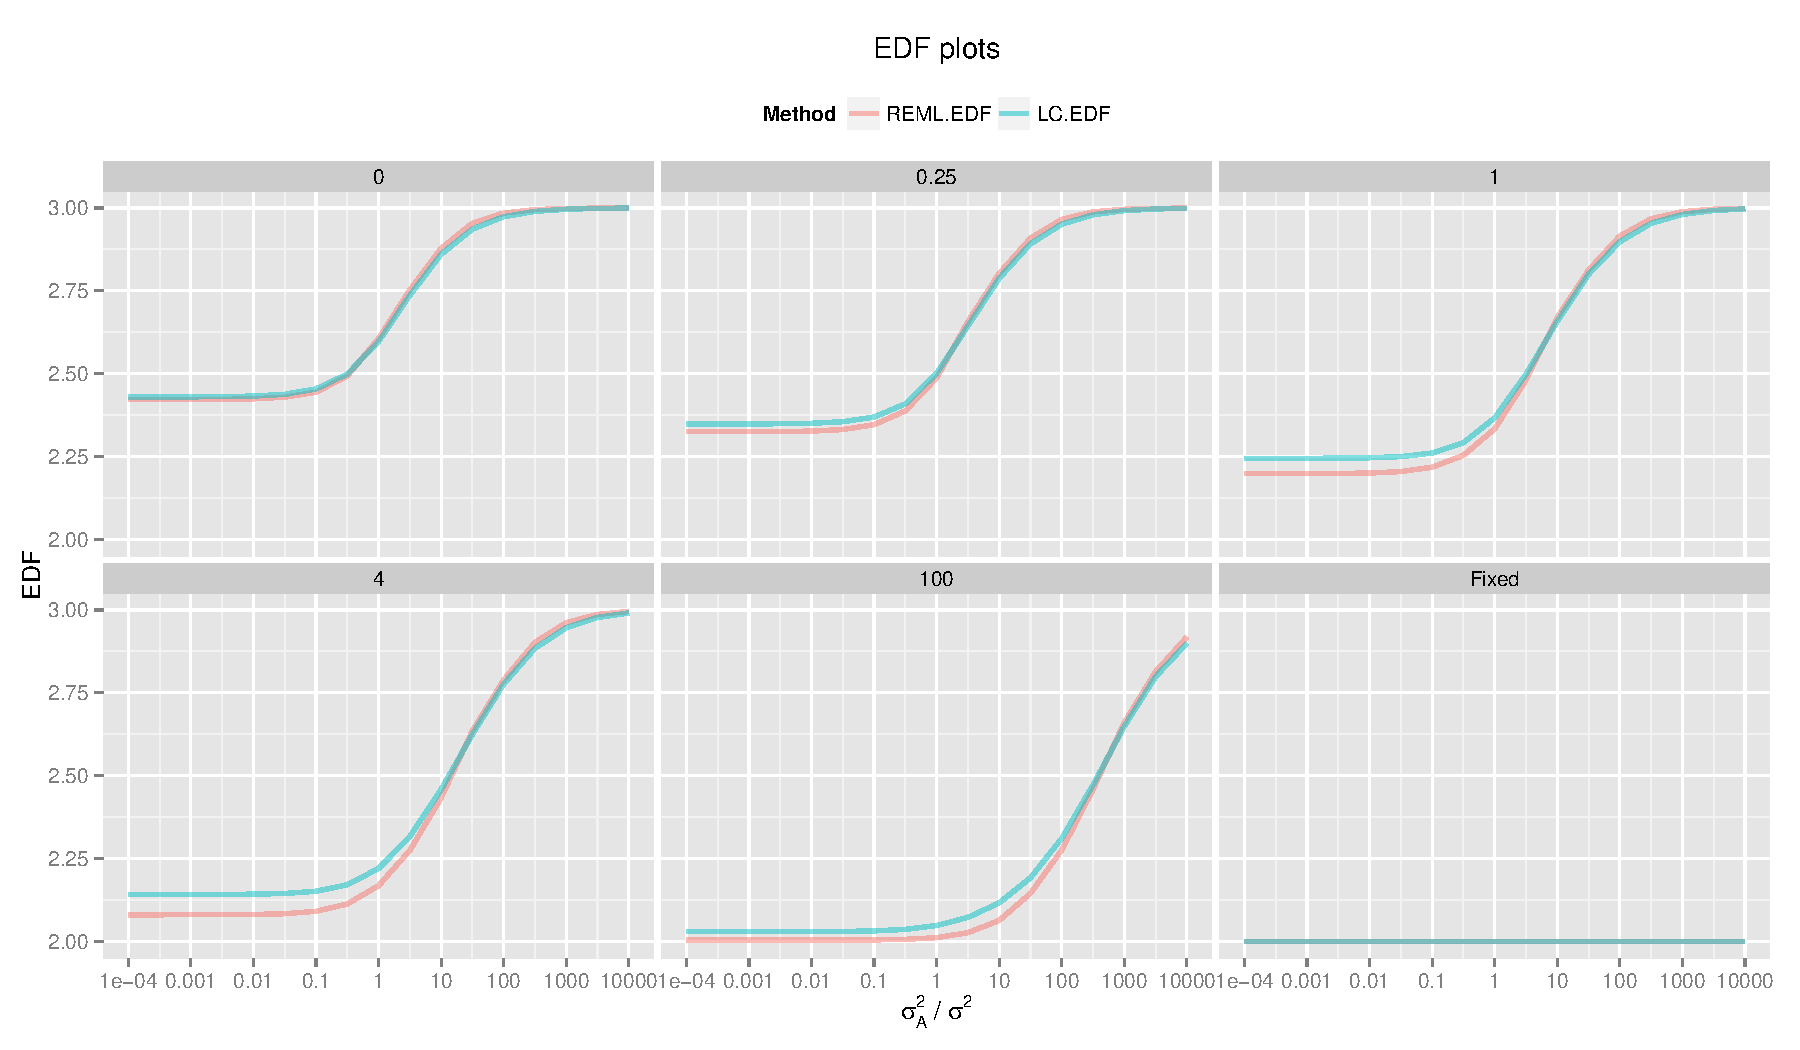
\includegraphics[width=1 \textwidth]{Graph/CRD232Tag4.pdf}
\caption{Plots of EDF from the negative VCs adjusted to zero}
\label{fig:EDFadjusted}
\end{figure}

\begin{figure}[ht]
\centering
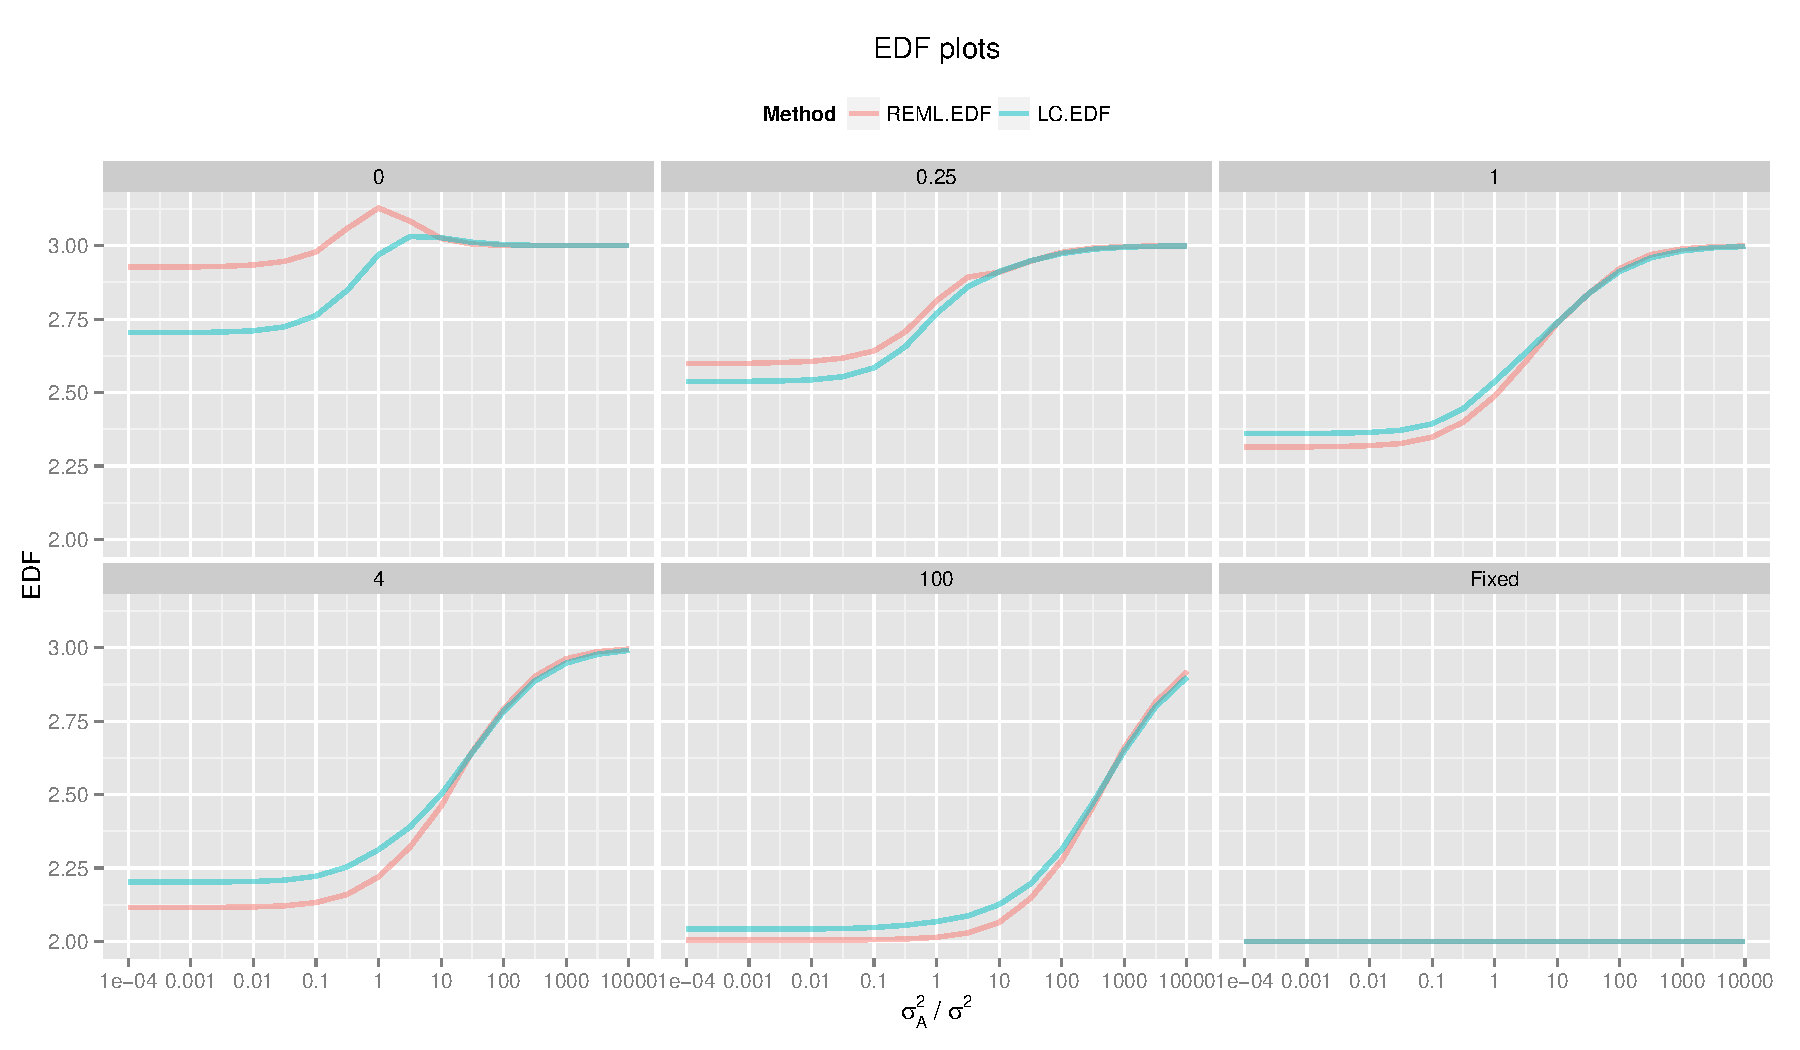
\includegraphics[width=1 \textwidth]{Graph/CRD232Tag4Unadjusted.pdf}
\caption{Plots of the EDF from unadjusted negative VCs.}
\label{fig:EDFunadjusted}
\end{figure}

The EDF plots of the adjusted VCs show that the EDF are higher when using the LC method compared to the REML method. If the VCs stays unadjusted, the EDF are only higher using the LC method compared to the REML method when Between Runs and Between Animals VCs estimates are low. The EDF from the adjusted VCs are always bound between 2 and 3, whereas the EDF from the unadjusted VCs can be as high as 3.18 if using the REML method at $\sigma^2_R = 0$ and $\sigma^2_A = 1$. The EDF from the unadjusted VCs always exceed the EDF from using adjusted VCs. This is because once the negative VCs are adjusted to zero, the estimated VCs can exceed expectations. The EDF can then be computed to be lower than expected. However, in theory, the EDF in the current example considered should not exceed 3, which is the maximum DF associated with the Between Animals stratum from the Phase 1 experiment. 

\subsection{Power analysis using the EDF}
The computed EDF can be used to conduct the tests for treatment effects. The residual MS also needs to be re-calculated using the VCs estimated from either the REML or LC method. Given that the residual DF increase from 2 to 3, the critical F-ratio at a significance of 0.05 decreases from 18.51282 to 10.12796. This should significantly increase the power of the F-test.  

The EDF plot shows that the EDF increase with the variation Between Animals. Recall the power analysis from the previous chapter that compared two designs with different residual DF and that showed which shoed that the power of the test decreased with increasing variation Between Animals. Consistent with that analysis, the main question here is whether, while inflation of EDF results from the inflation of the Between Animals variation and reduction of the Between Runs variation the estimated EDF are sufficiently high to increase the test power, as the Between Animals variation increases. 

Since treatment effects need to be tested they should be included in the simulated datasets. Hence, unlike the previous EDF plot generated from the simulated MS with the $\chi^2$ distribution, the following power plots are obtained from the simulated dataset generated using the normal distribution. The simulated datasets are generated with the true treatment mean groups of 0 and 4 and the true VCs remaining unchanged. The highest EDF between the LC and REML methods are used to conduct the test for treatment effects. The residual MS also needs to be adjusted based on the VCs estimates from the method that generates the highest EDF. The powers of the F-test are compared as between using the EDF with adjusted residual MS and using the original DF of 2 with residual MS from the ANOVA table. Moreover, the power plots based on the EDF computed from the adjusted and unadjusted VCs are presented in Figures~\ref{fig:PowerAdjusted} and ~\ref{fig:PowerUnadjusted}, respectively.

\begin{figure}[ht]
\centering
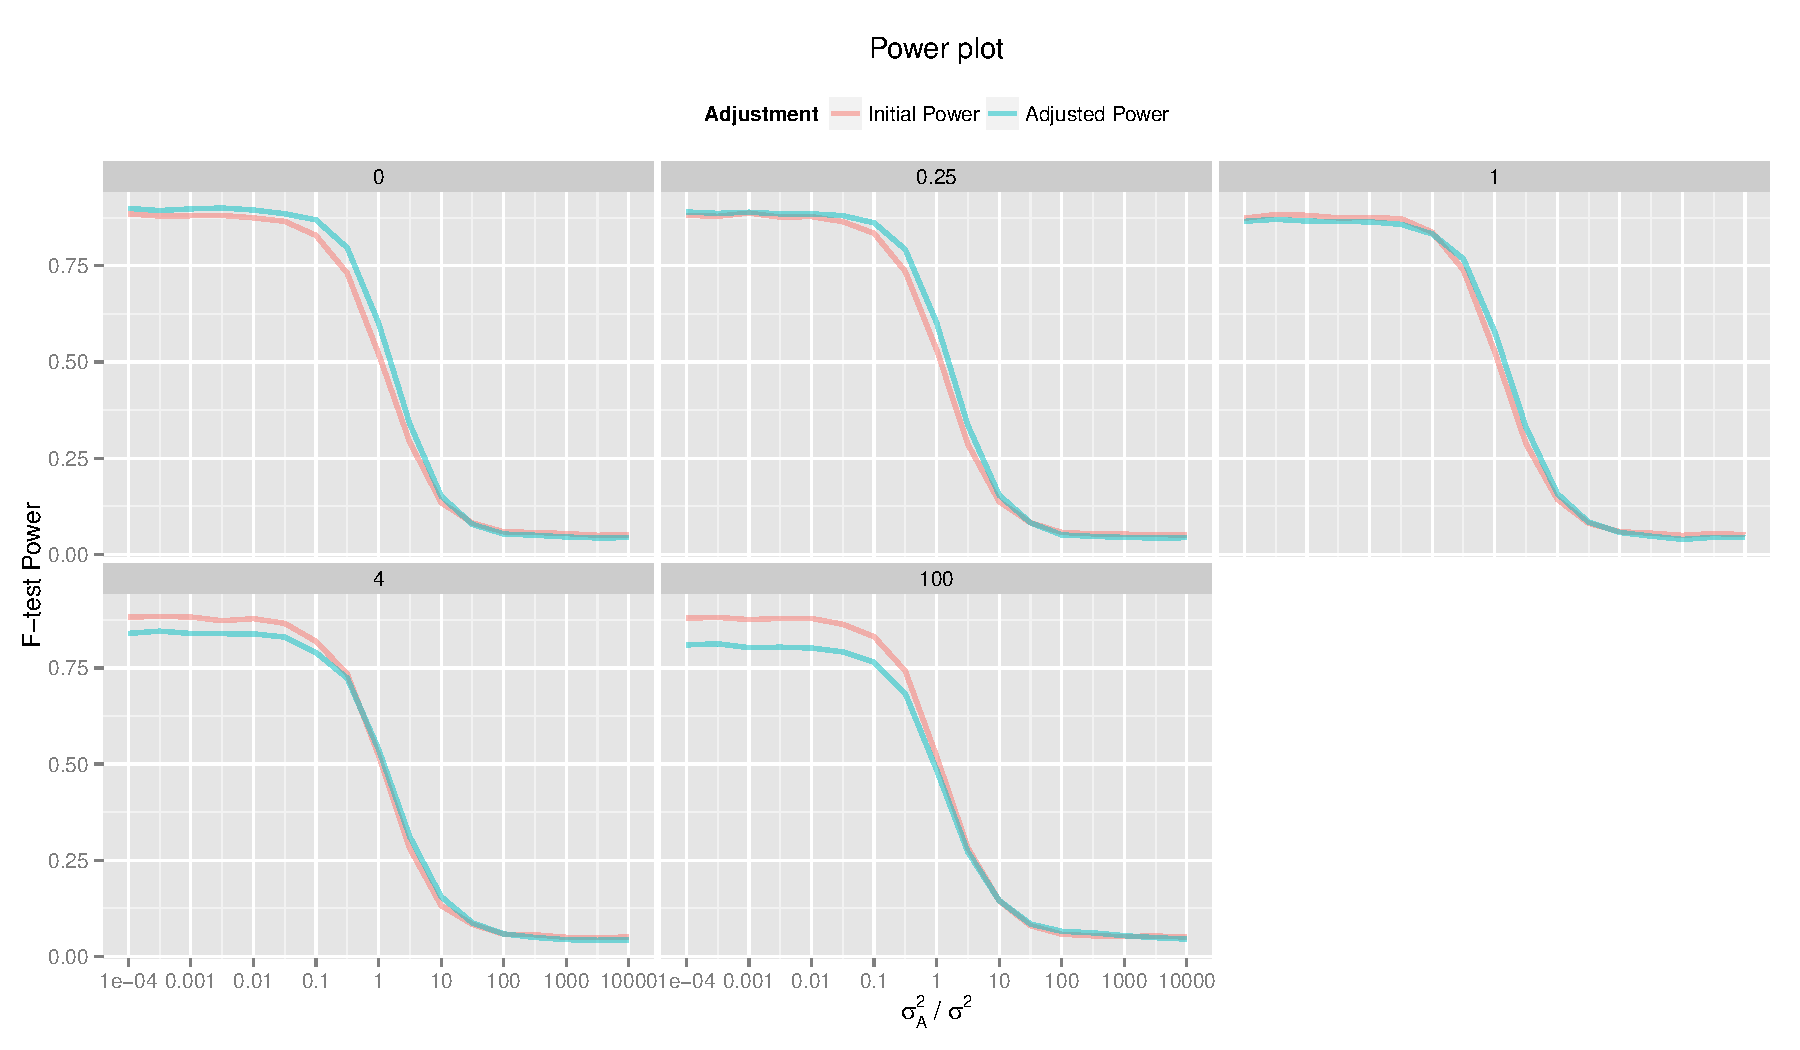
\includegraphics[width=1 \textwidth]{Graph/adjustZeroPowerEDF.pdf}
\caption{Plots of F-test power from the EDF of adjusted VCs.}
\label{fig:PowerAdjusted}
\end{figure}

When the negative VCs are adjusted to zero, F-test power can be greater when using original DF of 2 with the residual MS from the ANOVA table with low $\sigma_A^2$ and high $\sigma_R^2$. 

\begin{figure}[ht]
\centering
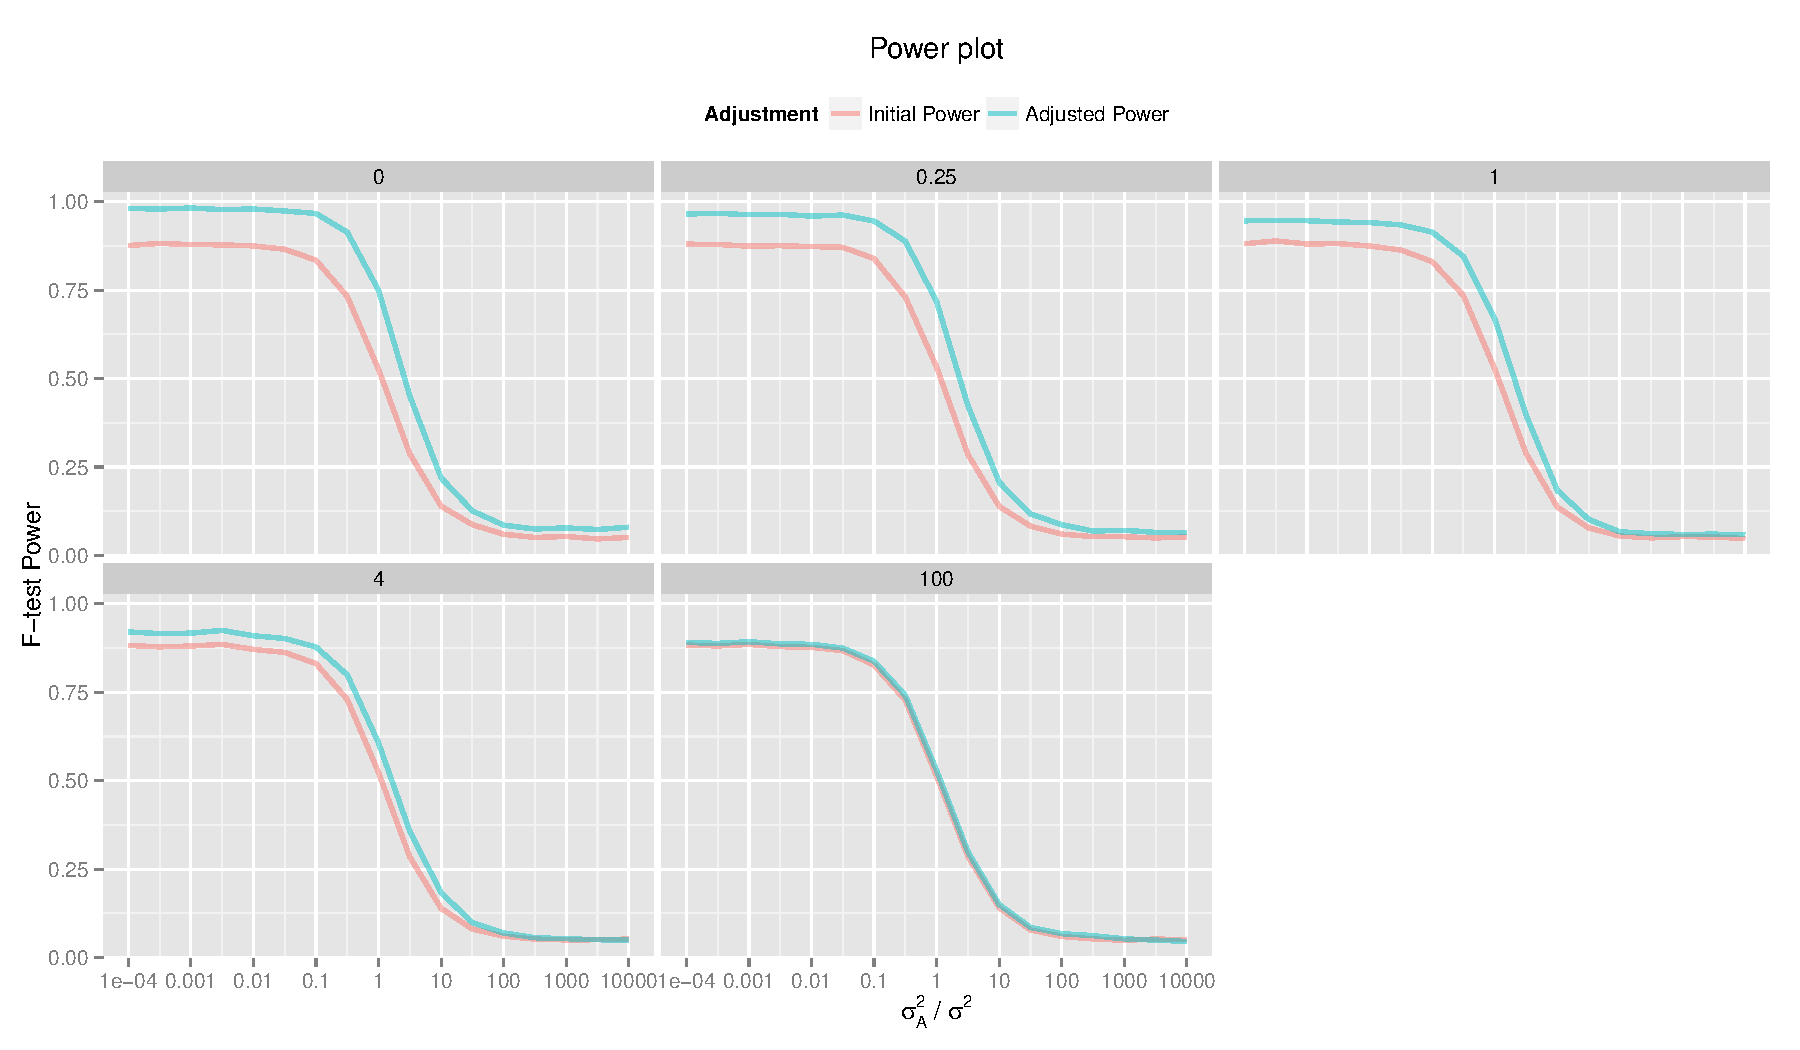
\includegraphics[width=1 \textwidth]{Graph/remainNegPowerEDF.pdf}
\caption{Plots of F-test power from EDF of unadjusted VCs.}
\label{fig:PowerUnadjusted}
\end{figure}

When the negative VCs remain unadjusted, the power of the F-test is better than when the negative VCs are adjusted to zero. This is because the negative VCs can lead to higher EDF, as shown in Figure~\ref{fig:EDFunadjusted}, as well as to lower estimated residual MS; thus, the power of the F-test increases. 

In conclusion, using the adjusted VCs is more accurate theoretically, because the EDF are always bounded within the expected range. However, the EDF can be skewed by the peak where the estimated $\sigma_A^2$ and $\sigma_R^2$ are both zero. For practical purposes, using the EDF with unadjusted VCs is better, because the mean of the adjusted VCs estimates tends to be higher than that of the unadjusted VCs estimates. Hence, the statistical power can be greatly increased, as shown in Figure~\ref{fig:PowerUnadjusted}. However, negative VCs estimates can cause the EDF to significantly exceed expectations, and thus the EDF will not be bounded within the expected range, as shown in Figure~\ref{fig:EDFunadjusted}.
  
\section{Comparing the EDF when Phase 1 is CRD}
This section compares the EDF obtained from the two-phase optimal designs found where the Phase 1 experiment is arranged in CRD. The main focus is on comparing four-plex and eight-plex experiments using the identical Phase 1 experiment. Three different cases are presented, showing that different sets of design parameters can work better depending on whether the four-plex or eight-plex experiment is used.

\subsection{First CRD example}
The first example experiment to be considered is the Phase 1 experiment with $v = 2$, $r_b = 6$ and $r_t = 2$. The theoretical ANOVA tables from the optimal design in which the Phase 2 experiments use 4 tags and 8 tags are presented in Tables~\ref{tab:ANOVAPhase1CRD11} and \ref{tab:ANOVAPhase1CRD12}, respectively. 
Based on these two theoretical ANOVA tables, the four-plex design is shown to be better, because it has both higher residual DF and treatment average efficiency factors than the eight-plex experiments for estimating treatment effects. 

\begin{table}[ht]
\centering
 \caption{Theoretical ANOVA table from the Phase 1 experiment arranged in CRD with $v = 2$ and $r_b = 6$, and the from the Phase 2 experiment using 4 tags}
 \begin{tabular}[t]{lrlll} 
 \toprule 
 \multicolumn{1}{l}{\textbf{Source of Variation}} & \multicolumn{1}{l}{\textbf{DF}} & \multicolumn{1}{l}{\textbf{EMS}}& \multicolumn{1}{l}{$\bm{E_{\gamma}}$}&\multicolumn{1}{l}{$\bm{E_{\tau}}$}\\ 
 \midrule 
 Between Runs &  &  & & \\ 
 \quad Between Animals & $2$ & $\sigma^2+2\sigma_{A}^2+4\sigma_{R}^2$ & & \\  \quad Within Animals & $3$ & $\sigma^2+4\sigma_{R}^2$ & & \\ \hline 
 Within Runs &  &  & & \\ 
 \quad Between Animals &  &  & & \\ 
 \quad \quad Tag & $1$ & $\sigma^2+2\sigma_{A}^2+6\theta_{\gamma}$ &$1$ & \\ 
 \quad \quad Treatment & $1$ & $\sigma^2+2\sigma_{A}^2+12\theta_{\tau}$ & & $1$\\ 
 \quad \quad Residual & $7$ & $\sigma^2+2\sigma_{A}^2$ & & \\ \hline 
 \quad Within Animals &  &  & & \\ 
 \quad \quad Tag & $2$ & $\sigma^2+6\theta_{\gamma}$ &$1$ & \\ 
 \quad \quad Residual & $7$ & $\sigma^2$ & & \\ 
 \bottomrule 
 \end{tabular} 
 \label{tab:ANOVAPhase1CRD11} 
\end{table} 

\begin{table}[ht]
\centering
 \caption{Theoretical ANOVA table from the Phase 1 experiment arranged in CRD with $v = 2$ and $r_b = 6$, and from the Phase 2 experiment with 8 tags}
 \begin{tabular}[t]{lrlll} 
 \toprule 
 \multicolumn{1}{l}{\textbf{Source of Variation}} & \multicolumn{1}{l}{\textbf{DF}} & \multicolumn{1}{l}{\textbf{EMS}}& \multicolumn{1}{l}{$\bm{E_{\gamma}}$}&\multicolumn{1}{l}{$\bm{E_{\tau}}$}\\ 
 \midrule 
 Between Runs &  &  & & \\ 
 \quad Between Animals & $1$ & $\sigma^2+2\sigma_{A}^2+8\sigma_{R}^2$ & & \\  \quad Within Animals & $1$ & $\sigma^2+8\sigma_{R}^2$ & & \\ \hline 
 Within Runs &  &  & & \\ 
 \quad Between Animals &  &  & & \\ 
 \quad \quad Tag & $3$ & $\sigma^2+2\sigma_{A}^2+3\theta_{\gamma}+ 1.33\theta_{\tau}$ &$1$ & $0.1111$\\ 
 \quad \quad Treatment & $1$ & $\sigma^2+2\sigma_{A}^2+10.67\theta_{\tau}$ & & $0.8889$\\ 
 \quad \quad Residual & $6$ & $\sigma^2+2\sigma_{A}^2$ & & \\ \hline 
 \quad Within Animals &  &  & & \\ 
 \quad \quad Tag & $4$ & $\sigma^2+3\theta_{\gamma}$ &$1$ & \\ 
 \quad \quad Residual & $7$ & $\sigma^2$ & & \\ 
 \bottomrule 
 \end{tabular} 
 \label{tab:ANOVAPhase1CRD12} 
\end{table} 

The plots of EDF are shown in Figure~\ref{fig:compare48CRD1}, which also shows that the EDF from the four-plex experiment always exceed those of the eight-plex experiment when the Phase 1 experiment is CRD with $v = 2$, $r_b = 6$ and $r_t = 2$. The EDF are at least 1 DF higher when the VCs of Between Animals are low. However, as the Between Animals VCs increase, the EDF can reach as high as 2 DF. 

\begin{figure}[ht]
\centering
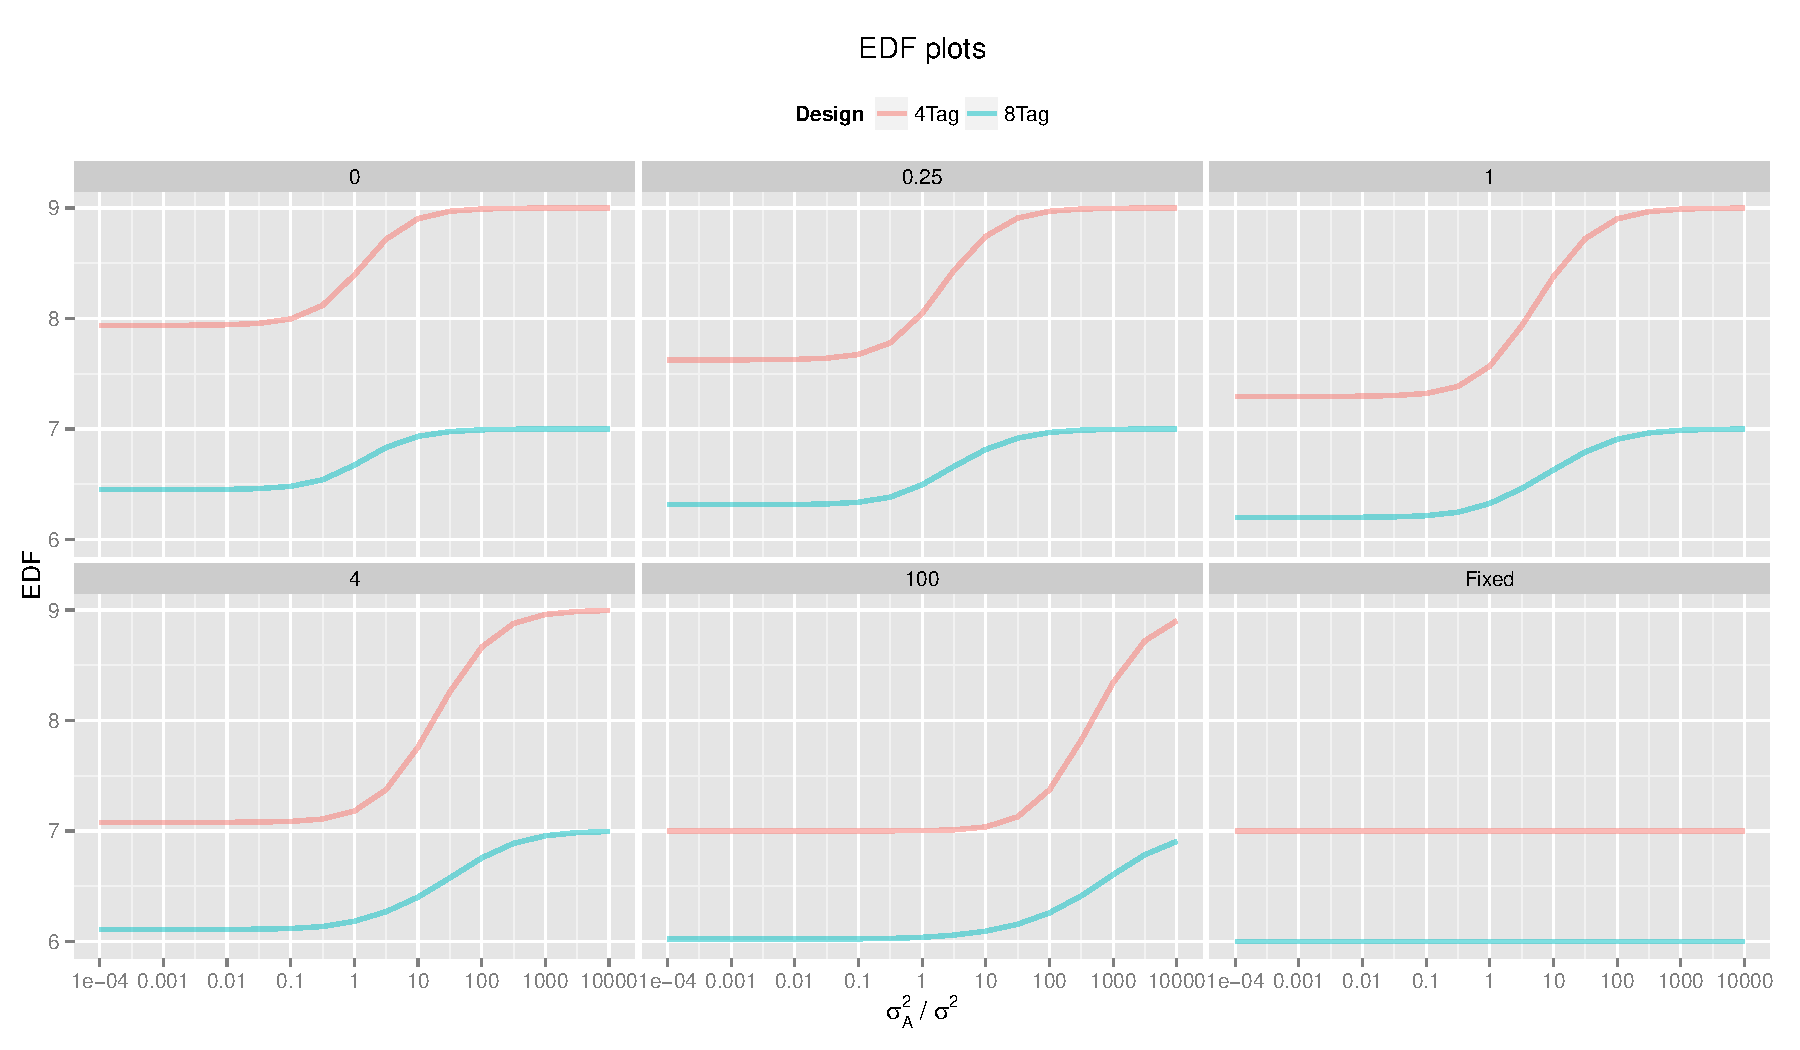
\includegraphics[width=1 \textwidth]{Graph/CRD262Tag4vsTag8.pdf}
\caption{Plots of EDF for experiments featuring $v = 2$ and $r_b = 6$, comparing four-plex and eight-plex systems}
\label{fig:compare48CRD1}
\end{figure}

This case is very typical when the Phase 1 experiment is CRD. This is because the four-plex experiments generally have 1 DF associated with tag effects in the Between Animals stratum, whereas the eight-plex experiments generally have 3 DF associated with tag effects in the Between Animals stratum. Hence, the EDF for the four-plex experiments can be up to 2 DF higher than for the eight-plex experiments for estimating the residual MS in the Between Animals strata. Therefore, for general cases, the four-plex experiments are better than the eight-plex experiments.

%When the comparisons can be done, the experiment using the four-plex system tends to have higher EDF, because fewer Between Animals DF are confounded with tag effects; thus as the variation Between Animals becomes much larger than that Between Runs, the EDF also increases. 

\subsection{Second CRD example}
The second example considers the experiment with $v = 4, r_b = 6$ and $r_t = 2$. The theoretical ANOVA tables from the optimal design where Phase 2 experiments use 4 tags and 8 tags are presented in Tables~\ref{tab:ANOVAPhase1CRD21} and \ref{tab:ANOVAPhase1CRD22}, respectively. 
Based on these two theoretical ANOVA tables, the design with 8 tags is shown to be better, because an eight-plex experiment has higher residual DF than a four-plex experiment for estimating treatment effects. However, the treatment average efficiency factor from the designs with the eight-plex experiment is $0.9623$, which is slightly lower than the $100\%$ for the four-plex experiment.  

\begin{table}[ht]
\centering
 \caption{Theoretical ANOVA table from the Phase 1 experiment arranged in CRD with $v = 4$ and $r_b = 6$, and from the Phase 2 experiment using 4 tags}
 \begin{tabular}[t]{lrlll} 
 \toprule 
 \multicolumn{1}{l}{\textbf{Source of Variation}} & \multicolumn{1}{l}{\textbf{DF}} & \multicolumn{1}{l}{\textbf{EMS}}& \multicolumn{1}{l}{$\bm{E_{\gamma}}$}&\multicolumn{1}{l}{$\bm{E_{\tau}}$}\\ 
 \midrule 
 Between Runs &  &  & & \\ 
 \quad Between Animals & $5$ & $\sigma^2+2\sigma_{A}^2+4\sigma_{R}^2$ & & \\  \quad Within Animals & $6$ & $\sigma^2+4\sigma_{R}^2$ & & \\ \hline 
 Within Runs &  &  & & \\ 
 \quad Between Animals &  &  & & \\ 
 \quad \quad Tag & $1$ & $\sigma^2+2\sigma_{A}^2+12\theta_{\gamma}$ &$1$ & \\ 
 \quad \quad Treatment & $3$ & $\sigma^2+2\sigma_{A}^2+12\theta_{\tau}$ & & $1$\\ 
 \quad \quad Residual & $14$ & $\sigma^2+2\sigma_{A}^2$ & & \\ \hline 
 \quad Within Animals &  &  & & \\ 
 \quad \quad Tag & $2$ & $\sigma^2+12\theta_{\gamma}$ &$1$ & \\ 
 \quad \quad Residual & $16$ & $\sigma^2$ & & \\ 
 \bottomrule 
 \end{tabular} 
 \label{tab:ANOVAPhase1CRD21} 
\end{table} 

\begin{table}[ht]
\centering
 \caption{Theoretical ANOVA table from the Phase 1 experiment arranged in CRD with $v = 4$ and $r_b = 6$, and from the Phase 2 experiment using 8 tags}
 \begin{tabular}[t]{lrlll} 
 \toprule 
 \multicolumn{1}{l}{\textbf{Source of Variation}} & \multicolumn{1}{l}{\textbf{DF}} & \multicolumn{1}{l}{\textbf{EMS}}& \multicolumn{1}{l}{$\bm{E_{\gamma}}$}&\multicolumn{1}{l}{$\bm{E_{\tau}}$}\\ 
 \midrule 
 Between Runs &  &  & & \\ 
 \quad Between Animals & $2$ & $\sigma^2+2\sigma_{A}^2+8\sigma_{R}^2$ & & \\  \quad Within Animals & $3$ & $\sigma^2+8\sigma_{R}^2$ & & \\ \hline 
 Within Runs &  &  & & \\ 
 \quad Between Animals &  &  & & \\ 
 \quad \quad Tag & $3$ & $\sigma^2+2\sigma_{A}^2+6\theta_{\gamma}+ 0.67\theta_{\tau}$ &$1$ & $0.0556$\\ 
 \quad \quad Treatment & $3$ & $\sigma^2+2\sigma_{A}^2+11.55\theta_{\tau}$ & & $0.9623$\\ 
 \quad \quad Residual & $15$ & $\sigma^2+2\sigma_{A}^2$ & & \\ \hline 
 \quad Within Animals &  &  & & \\ 
 \quad \quad Tag & $4$ & $\sigma^2+6\theta_{\gamma}$ &$1$ & \\ 
 \quad \quad Residual & $17$ & $\sigma^2$ & & \\ 
 \bottomrule 
 \end{tabular} 
 \label{tab:ANOVAPhase1CRD22} 
\end{table} 

Figure~\ref{fig:compare44CRD} shows the plot of EDF. The EDF from the four-plex experiments always exceed those from the eight-plex experiments when the Between Runs VCs are zero. Otherwise, the EDF from the eight-plex experiment can exceed those for the four-plex experiment with low Between Animal VCs. However, as the Between Animals VCs increase, the EDF of four-plex experiments become better than for the experiment with 8 tags. Thus, the eight-plex experiments are only better than the four-plex experiments with low Between Animals VCs and high Between Runs VCs estimates.

\begin{figure}[ht]
\centering
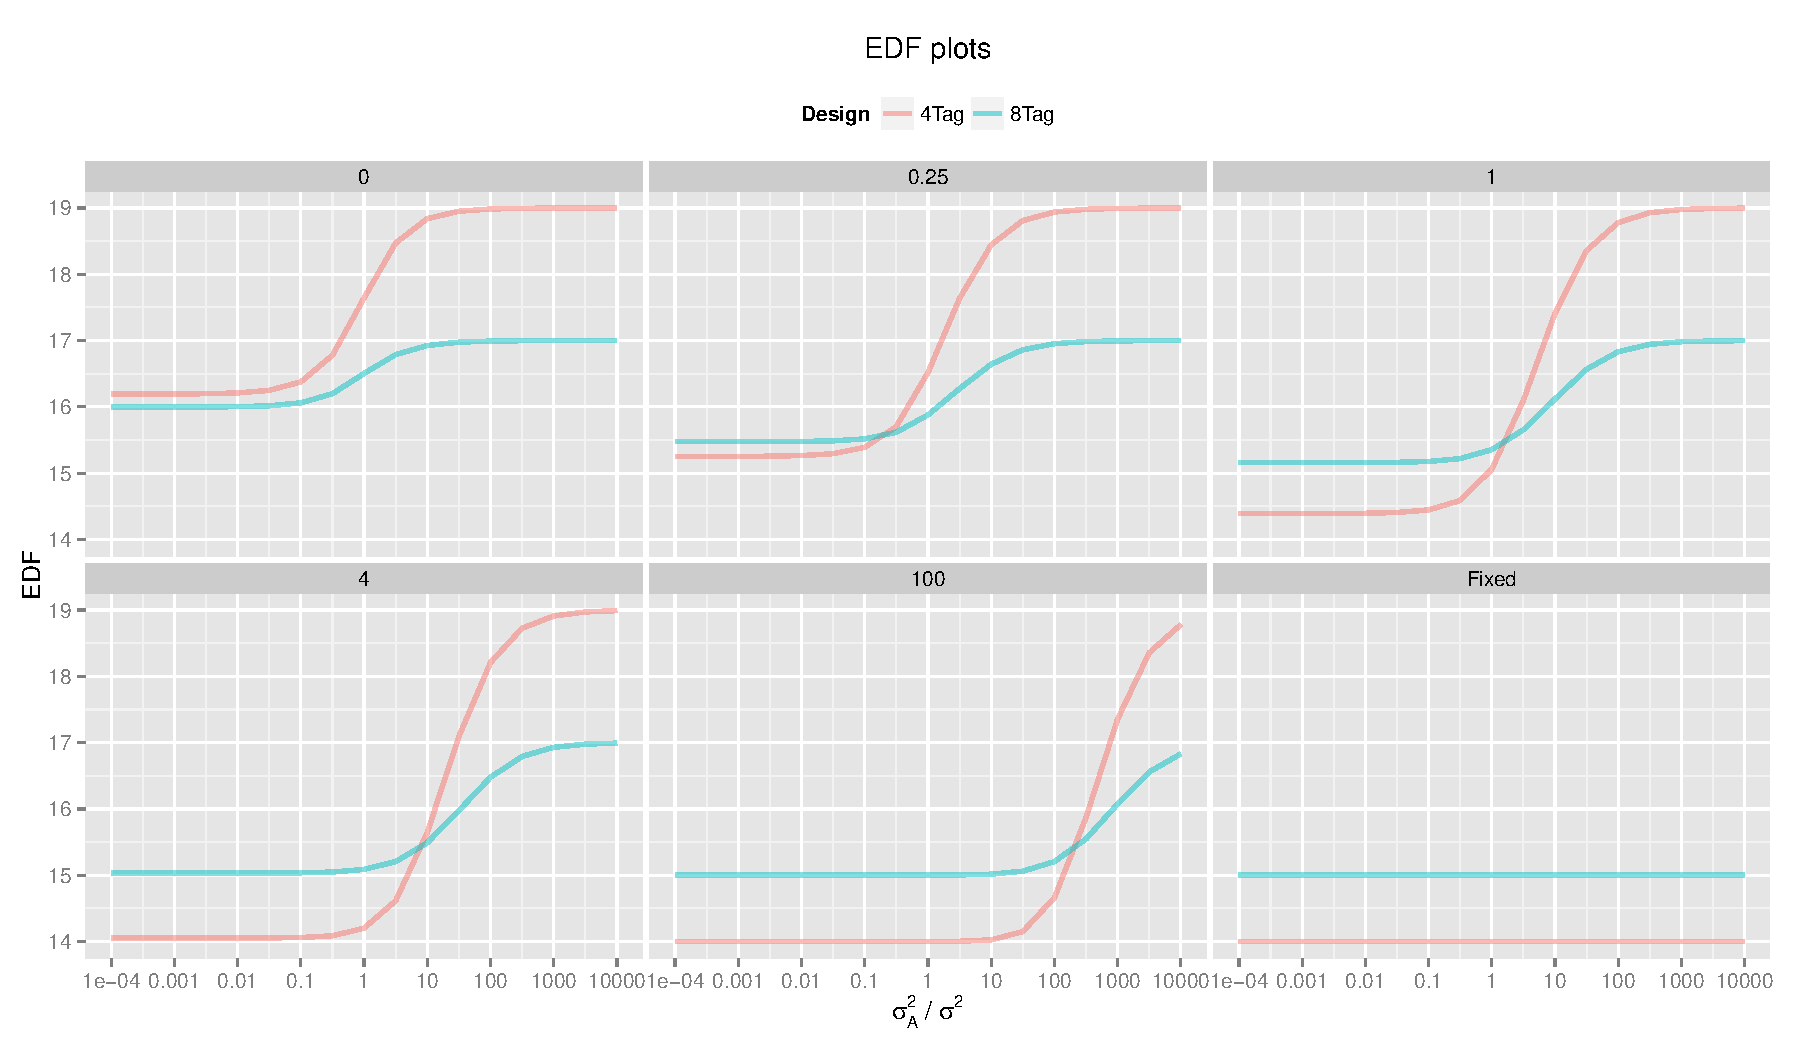
\includegraphics[width=1 \textwidth]{Graph/CRD462Tag4vsTag8.pdf}
\caption{Plots of EDF for experiments featuring $v = 4$ and $r_b = 6$, comparing four-plex and eight-plex systems}
\label{fig:compare44CRD}
\end{figure}

This type of situation occurs given high $r_b$ in the Phase 1 experiment. Due to the disconnectedness in the allocation of animals to runs, some DF associated with the Between Animals stratum can be in the Between Runs stratum. As the $r_b$ increases, the four-plex experiments will have more DF associated with animals in the Between Runs stratum than the eight-plex experiments do. This is because each run of the four-plex experiment can measure only up to 4 samples. 

However, the residual DF increases with an increase in the biological replicate. For this example with $v = 4, r_b = 6$ and $r_t = 2$, the critical F-ratios for $(3,19)$ and $(3,14)$ DF are 3.12735 and 3.343889, respectively, at a significance level at 0.05. Thus, the power of the F-test should not differ significantly between these two designs. Therefore, these two designs should be equally effective under different Between Runs and Between Animals VCs.

\subsection{Third CRD example}
The third example considers the experiment with $v = 8, r_b = 2$ and $r_t = 2$. The theoretical ANOVA tables from the optimal design where Phase 2 experiments use 4 tags and 8 tags are presented in Tables~\ref{tab:ANOVAPhaseCRD31} and \ref{tab:ANOVAPhaseCRD32}, respectively. 
Based on these two theoretical ANOVA tables, these two designs are equally effective as regards both higher residual DF and treatment average efficiency factors. 

\begin{table}[ht]
\centering
 \caption{Theoretical ANOVA table from the Phase 1 experiment arranged in CRD with $v = 8$ and $r_b = 2$, and from the Phase 2 experiment using 4 tags.}
 \begin{tabular}[t]{lrlll} 
 \toprule 
 \multicolumn{1}{l}{\textbf{Source of Variation}} & \multicolumn{1}{l}{\textbf{DF}} & \multicolumn{1}{l}{\textbf{EMS}}& \multicolumn{1}{l}{$\bm{E_{\gamma}}$}&\multicolumn{1}{l}{$\bm{E_{\tau}}$}\\ 
 \midrule 
 Between Runs &  &  & & \\ 
 \quad Between Animals &  &  & & \\ 
 \quad \quad Treatment & $3$ & $\sigma^2+2\sigma_{A}^2+4\sigma_{R}^2+1.2\theta_{\tau}$ & & $0.3$\\ 
 \quad Within Animals & $4$ & $\sigma^2+4\sigma_{R}^2$ & & \\ \hline 
 Within Run &  &  & & \\ 
 \quad Between Animals &  &  & & \\ 
 \quad \quad Tag & $1$ & $\sigma^2+2\sigma_{A}^2+8\theta_{\gamma}$ &$1$ & \\ 
 \quad \quad Treatment & $7$ & $\sigma^2+2\sigma_{A}^2+ 3.23\theta_{\tau}$ & & $0.8077$\\ 
 \quad \quad Residual & $4$ & $\sigma^2+2\sigma_{A}^2$ & & \\ \hline 
 \quad Within Animals &  &  & & \\ 
 \quad \quad Tag & $2$ & $\sigma^2+8\theta_{\gamma}$ &$1$ & \\ 
 \quad \quad Residual & $10$ & $\sigma^2$ & & \\ 
 \bottomrule 
 \end{tabular} 
 \label{tab:ANOVAPhaseCRD31} 
\end{table} 

\begin{table}[ht]
\centering
 \caption{Theoretical ANOVA table from the Phase 1 experiment arranged in CRD with $v = 8$ and $r_b = 2$ and the Phase 2 experiment using 8 tags.}
 \begin{tabular}[t]{lrlll} 
 \toprule 
 \multicolumn{1}{l}{\textbf{Source of Variation}} & \multicolumn{1}{l}{\textbf{DF}} & \multicolumn{1}{l}{\textbf{EMS}}& \multicolumn{1}{l}{$\bm{E_{\gamma}}$}&\multicolumn{1}{l}{$\bm{E_{\tau}}$}\\ 
 \midrule 
 Between Runs &  &  & & \\ 
 \quad Between Animals & $1$ & $\sigma^2+2\sigma_{A}^2+8\sigma_{R}^2$ & & \\ 
 \quad Within Animals & $2$ & $\sigma^2+8\sigma_{R}^2$ & & \\ \hline 
 Within Runs &  &  & & \\ 
 \quad Between Animals &  &  & & \\ 
 \quad \quad Tag & $3$ & $\sigma^2+2\sigma_{A}^2+4\theta_{\gamma}+1.2\theta_{\tau}$ &$1$ &  $0.3$\\ 
 \quad \quad Treatment & $7$ & $\sigma^2+2\sigma_{A}^2+3.23\theta_{\tau}$ & & $0.8077$\\ 
 \quad \quad Residual & $4$ & $\sigma^2+2\sigma_{A}^2$ & & \\ \hline 
 \quad Within Animals &  &  & & \\ 
 \quad \quad Tag & $4$ & $\sigma^2+4\theta_{\gamma}$ &$1$ & \\ 
 \quad \quad Residual & $10$ & $\sigma^2$ & & \\ 
 \bottomrule 
 \end{tabular} 
 \label{tab:ANOVAPhaseCRD32} 
\end{table} 

The plot of EDF can be expressed as in Figure~\ref{fig:compare82CRD}, which shows that the EDF from the eight-plex experiment are higher than those from the four-plex experiment, especially when the VCs estimates are low for Between Runs and high for Between Animals. The EDF can be the same for the two designs with low Between Animals VCs and high  Between Runs VCs. Therefore, when the Phase 1 experiment is CRD with $v = 5$, $r_b = 2$ and $r_t = 2$, the eight-plex experiment is preferable.

\begin{figure}[ht]
\centering
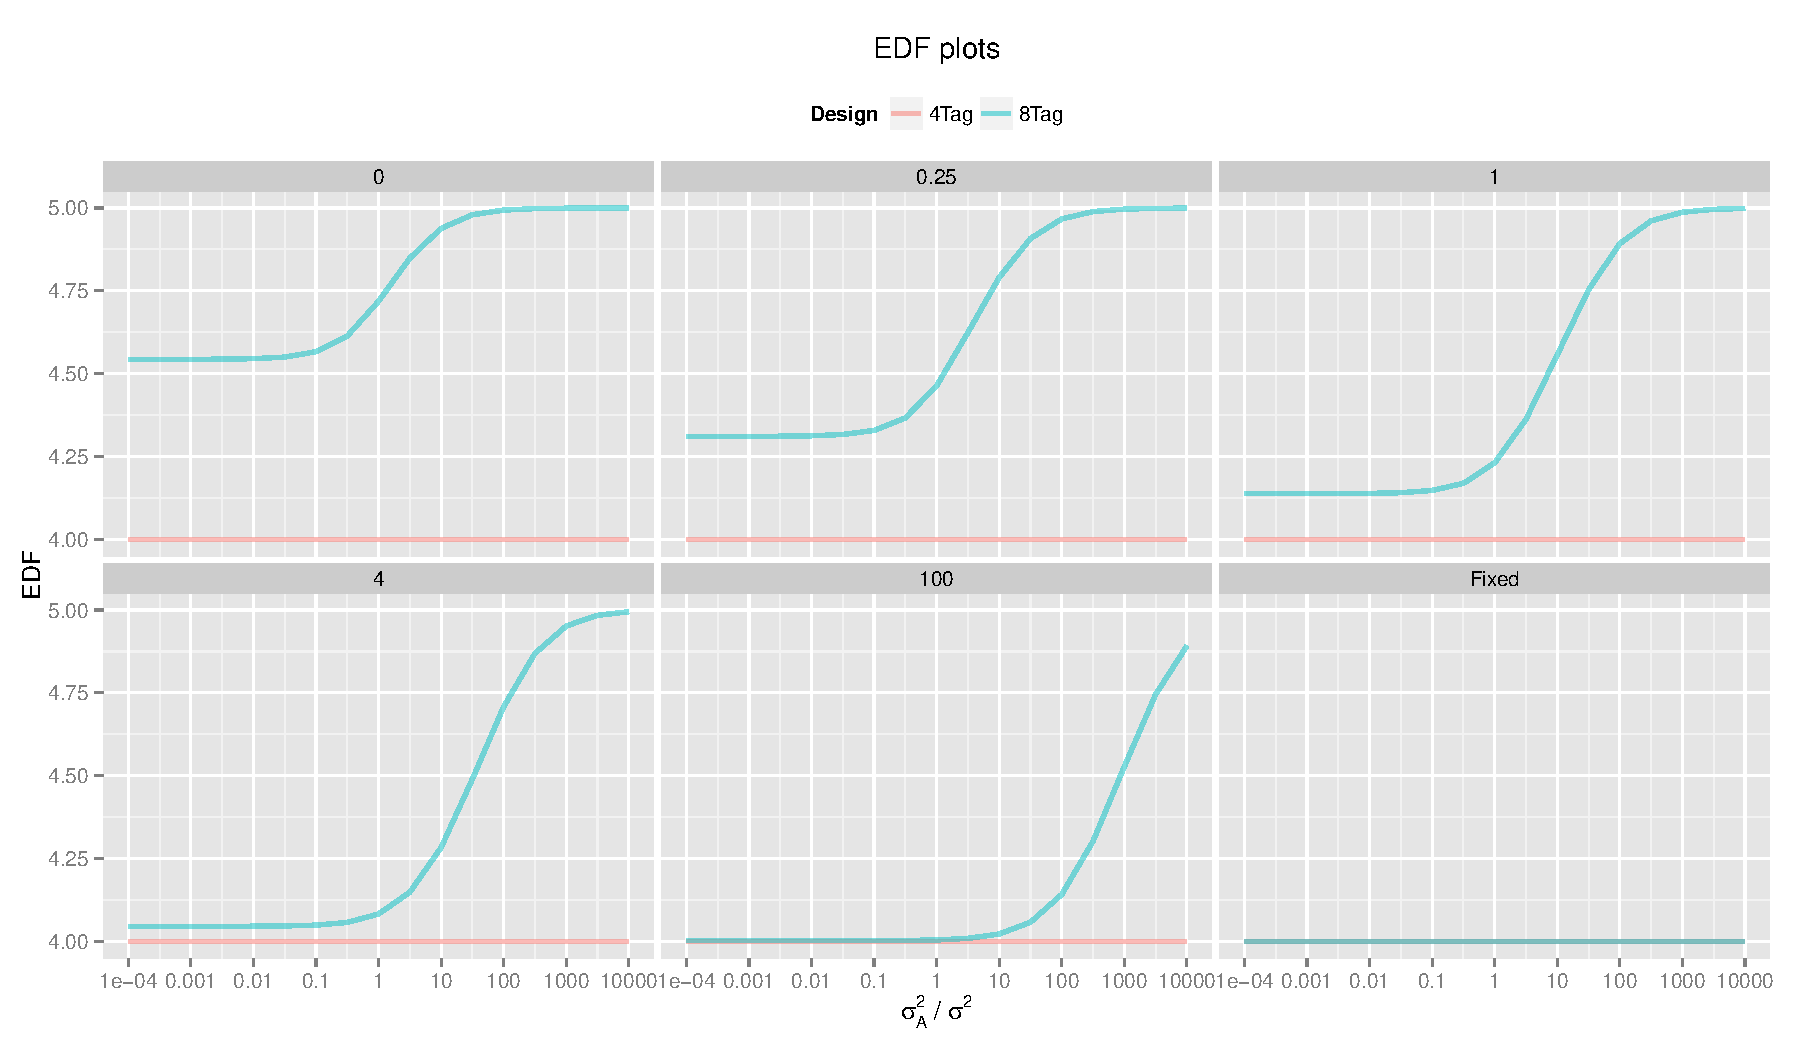
\includegraphics[width=1 \textwidth]{Graph/CRD822Tag4vsTag8.pdf}
\caption{Plots of EDF for experiments featuring $v = 8$ and $r_b = 2$ comparing four-plex and eight-plex systems}
\label{fig:compare82CRD}
\end{figure}

This example shows that the eight-plex experiment is better only when comparing eight different treatments in the Phase 1 experiment. As shown from the theoretical ANOVA table in Table~\ref{tab:ANOVAPhaseCRD31}, some treatment information are in the Between Runs stratum, which also confounds all 3 DF associated with the Between Animals stratum. Thus, it is impossible to recover these 3 DF using the method presented in this chapter. Therefore, the EDF for the four-plex experiment remain 4 with different VCs estimates. As for the experiment with 8 tags, the theoretical ANOVA table in Table~\ref{tab:ANOVAPhaseCRD32} shows that the treatments are not confounded with runs; hence, the 1 DF associated with the Between Animals stratum in the Between Runs can be recovered with high Between Animals VCs and low Between Runs VCs. Therefore, the eight-plex experiment is better for comparing eight treatments.  

To summarise: When the Phase 1 experiment is CRD, it is generally preferable to use the four-plex system with a small number of biological replicates. As the number of biological replicates increases, the eight-plex system can have higher EDF than the four-plex system with low Between Animals VCs and high Between Runs VCs. However, the power of the F-test should not differ significantly, since the critical F-ratio is similar for both designs. Considering time and budget constraints, the eight-plex system should be preferred, because it can measure more samples in the same run. The eight-plex experiment should always be used when comparing eight treatments, because the treatments are orthogonal to runs, which maximises the animal information. 

\section{Comparing the EDF when Phase 1 experiment is RCBD}
\label{sec:expRCBD}
This section compares the EDF obtained from the two-phase optimal designs found where the Phase 1 experiment is arranged in RCBD. The Phase 1 experiment uses cages as barriers to separate the sets of animals. Regarding this cage component, recall from the chapter on searching for an optimal design that the initial designs can confound cages more with either tags or runs. In addition to comparing these two initial designs, the designs from four-plex and eight-plex experiments can also be compared. An example where the Phase 1 experiment is arranged in RCBD illustrates how cage allocation to runs and tags can affect the EDF with different VCs estimates.  

\subsection{The RCBD example} 
The example experiment to be consider feature a Phase 1 experiment consisting of $v = 4$, $r_b = 4, n_B  = 4$ and $r_t = 2$. Four different two-phase designs can be compared using the same Phase 1 experiment. The theoretical ANOVA tables for each of these four designs are presented in Tables~\ref{tab:ANOVAPhase1RCBD1}, \ref{tab:ANOVAPhase1RCBD2}, \ref{tab:ANOVAPhase1RCBD3} and \ref{tab:ANOVAPhase1RCBD4}. Based on these four theoretical ANOVA tables, Tables~\ref{tab:ANOVAPhase1RCBD1} and \ref{tab:ANOVAPhase1RCBD4} appear to perform equally well, with maximum residual DF of 8 and $100\%$ of the treatment information in the Between Animals Within Cages Within Runs stratum. However, as shown from the second CRD example, the EDF may be better in different designs with different VCs estimates. Hence, the EDF need to be assessed from these four designs. 

\begin{table}[ht]
\centering
 \caption{Theoretical ANOVA table from the Phase 1 experiment arranged in RCBD where $v = 4$ and $r_b = 4$, and with from the Phase 2 experiment using 4 tags and an initial design in which cage is confounded more with runs}
 \begin{tabular}[t]{lrlll} 
 \toprule 
 \multicolumn{1}{l}{\textbf{Source of Variation}} & \multicolumn{1}{l}{\textbf{DF}} & \multicolumn{1}{l}{\textbf{EMS}}& \multicolumn{1}{l}{$\bm{E_{\gamma}}$}&\multicolumn{1}{l}{$\bm{E_{\tau}}$}\\ 
 \midrule 
 Between Runs &  &  & & \\ 
 \quad Between Cages & $3$ & $\sigma^2+2\sigma_{A}^2+8\sigma_{B}^2+4\sigma_{R}^2$ & & \\  
 \quad Within Animals Within Cages & $4$ & $\sigma^2+4\sigma_{R}^2$ & & \\ \hline 
 Within Runs &  &  & & \\ 
 \quad Between Animals Within Cages &  &  & & \\ 
 \quad \quad Tag & $1$ & $\sigma^2+2\sigma_{A}^2+8\theta_{\gamma}$ &$1$ & \\ 
 \quad \quad Treatment & $3$ & $\sigma^2+2\sigma_{A}^2+8\theta_{\tau}$ & & $1$\\ 
 \quad \quad Residual & $8$ & $\sigma^2+2\sigma_{A}^2$ & & \\ \hline 
 \quad Within Animals Within Cages &  &  & & \\ 
 \quad \quad Tag & $2$ & $\sigma^2+8\theta_{\gamma}$ &$1$ & \\ 
 \quad \quad Residual & $10$ & $\sigma^2$ & & \\ 
 \bottomrule 
 \end{tabular} 
 \label{tab:ANOVAPhase1RCBD1} 
\end{table} 

\begin{table}[ht]
\centering
 \caption{Theoretical ANOVA table from the Phase 1 experiment arranged in RCBD and where $v = 4$ and $r_b = 4$, and from the Phase 2 experiment using four tags and an initial design in which cage is confounded more with tags.}
 \begin{tabular}[t]{lrlll} 
 \toprule 
 \multicolumn{1}{l}{\textbf{Source of Variation}} & \multicolumn{1}{l}{\textbf{DF}} & \multicolumn{1}{l}{\textbf{EMS}}& \multicolumn{1}{l}{$\bm{E_{\gamma}}$}&\multicolumn{1}{l}{$\bm{E_{\tau}}$}\\ 
 \midrule 
 Between Runs &  &  & & \\ 
 \quad Between Cages & $1$ & $\sigma^2+2\sigma_{A}^2+8\sigma_{B}^2+4\sigma_{R}^2$ & & \\  
 \quad Between Animals Within Cages & $2$ & $\sigma^2+2\sigma_{A}^2+4\sigma_{R}^2$ & & \\  
 \quad Within Animals Within Cages & $4$ & $\sigma^2+4\sigma_{R}^2$ & & \\ \hline 
 Within Runs &  &  & & \\ 
 \quad Between Cages &  &  & & \\ 
 \quad \quad Tag & $1$ & $\sigma^2+2\sigma_{A}^2+8\sigma_{B}^2+8\theta_{\gamma}$ &$1$ & \\ 
 \quad \quad Residual & $1$ & $\sigma^2+2\sigma_{A}^2+8\sigma_{B}^2$ & & \\ \hline 
 \quad Between Animals Within Cages &  &  & & \\ 
 \quad \quad Treatment & $3$ & $\sigma^2+2\sigma_{A}^2+8\theta_{\tau}$ & & $1$\\ 
 \quad \quad Residual & $7$ & $\sigma^2+2\sigma_{A}^2$ & & \\ \hline 
 \quad Within Animals Within Cages &  &  & & \\ 
 \quad \quad Tag & $2$ & $\sigma^2+8\theta_{\gamma}$ &$1$ & \\ 
 \quad \quad Residual & $10$ & $\sigma^2$ & & \\ 
 \bottomrule 
 \end{tabular} 
 \label{tab:ANOVAPhase1RCBD2} 
\end{table} 

\begin{table}[ht]
\centering
 \caption{Theoretical ANOVA table from the Phase 1 experiment arranged in RCBD and where $v = 4$ and $r_b = 4$, and from the Phase 2 experiment using 8 tags and an initial design in which cage is confounded more with runs.}
 \begin{tabular}[t]{lrlll} 
 \toprule 
 \multicolumn{1}{l}{\textbf{Source of Variation}} & \multicolumn{1}{l}{\textbf{DF}} & \multicolumn{1}{l}{\textbf{EMS}}& \multicolumn{1}{l}{$\bm{E_{\gamma}}$}&\multicolumn{1}{l}{$\bm{E_{\tau}}$}\\ 
 \midrule 
 Between Runs &  &  & & \\ 
 \quad Between Cages & $1$ & $\sigma^2+2\sigma_{A}^2+8\sigma_{B}^2+8\sigma_{R}^2$ & & \\  
 \quad Within Animals Within Cages & $2$ & $\sigma^2+8\sigma_{R}^2$ & & \\ \hline 
 Within Runs &  &  & & \\ 
 \quad Between Cages &  &  & & \\ 
 \quad \quad Tag & $1$ & $\sigma^2+2\sigma_{A}^2+8\sigma_{B}^2+4\theta_{\gamma}$ &$1$ & \\ 
 \quad \quad Residual & $1$ & $\sigma^2+2\sigma_{A}^2+8\sigma_{B}^2$ & & \\ \hline 
 \quad Between Animals Within Cages &  &  & & \\ 
 \quad \quad Tag & $2$ & $\sigma^2+2\sigma_{A}^2+4\theta_{\gamma}$ &$1$ & \\ 
 \quad \quad Treatment & $3$ & $\sigma^2+2\sigma_{A}^2+8\theta_{\tau}$ & & $1$\\ 
 \quad \quad Residual & $7$ & $\sigma^2+2\sigma_{A}^2$ & & \\ \hline 
 \quad Within Animals Within Cages &  &  & & \\ 
 \quad \quad Tag & $4$ & $\sigma^2+4\theta_{\gamma}$ &$1$ & \\ 
 \quad \quad Residual & $10$ & $\sigma^2$ & & \\ 
 \bottomrule 
 \end{tabular} 
 \label{tab:ANOVAPhase1RCBD3} 
\end{table} 

\begin{table}[ht]
\centering
 \caption{Theoretical ANOVA table from the Phase 1 experiment arranged in RCBD where $v = 4$ and $r_b = 4$, and from the Phase 2 experiment using 8 tags and an initial design in which cage is confounded more with tags.}
 \begin{tabular}[t]{lrlll} 
 \toprule 
 \multicolumn{1}{l}{\textbf{Source of Variation}} & \multicolumn{1}{l}{\textbf{DF}} & \multicolumn{1}{l}{\textbf{EMS}}& \multicolumn{1}{l}{$\bm{E_{\gamma}}$}&\multicolumn{1}{l}{$\bm{E_{\tau}}$}\\ 
 \midrule 
 Between Runs &  &  & & \\ 
 \quad Between Animals Within Cages & $1$ & $\sigma^2+2\sigma_{A}^2+8\sigma_{R}^2$ & & \\ 
 \quad Within Animals Within Cages & $2$ & $\sigma^2+8\sigma_{R}^2$ & & \\ \hline 
 Within Runs &  &  & & \\ 
 \quad Between Cages &  &  & & \\ 
 \quad \quad Tag & $3$ & $\sigma^2+2\sigma_{A}^2+8\sigma_{B}^2+4\theta_{\gamma}$ &$1$ & \\ \hline 
 \quad Between Animals Within Cages &  &  & & \\ 
 \quad \quad Treatment & $3$ & $\sigma^2+2\sigma_{A}^2+8\theta_{\tau}$ & & $1$\\ 
 \quad \quad Residual & $8$ & $\sigma^2+2\sigma_{A}^2$ & & \\ \hline 
 \quad Within Animals Within Cages &  &  & & \\ 
 \quad \quad Tag & $4$ & $\sigma^2+4\theta_{\gamma}$ &$1$ & \\ 
 \quad \quad Residual & $10$ & $\sigma^2$ & & \\ 
 \bottomrule 
 \end{tabular} 
 \label{tab:ANOVAPhase1RCBD4} 
\end{table} 

The first comparison of the EDF is between the two initial designs using the four-plex experiments. Figure~\ref{fig:RCBD442Tag4EDF} plots the EDF. The design in which cages are confounded more with runs is indicated by the pink line for which the EDF are always 8. This phenomenon can be explained by the theoretical ANOVA table in Table~\ref{tab:ANOVAPhase1RCBD1}, where the Between Runs stratum does not contain the Between Animals Within Cages stratum. Another explanation is that the between VCs estimates can only be derived from the Within Runs stratum. Back to Figure~\ref{fig:RCBD442Tag4EDF}, the remaining six colours represent the EDF with different VCs Between Cages, these plots show the Between Cages VCs can only affect the EDF when the Between Animals VCs are small.  

\begin{figure}[h!]
\centering
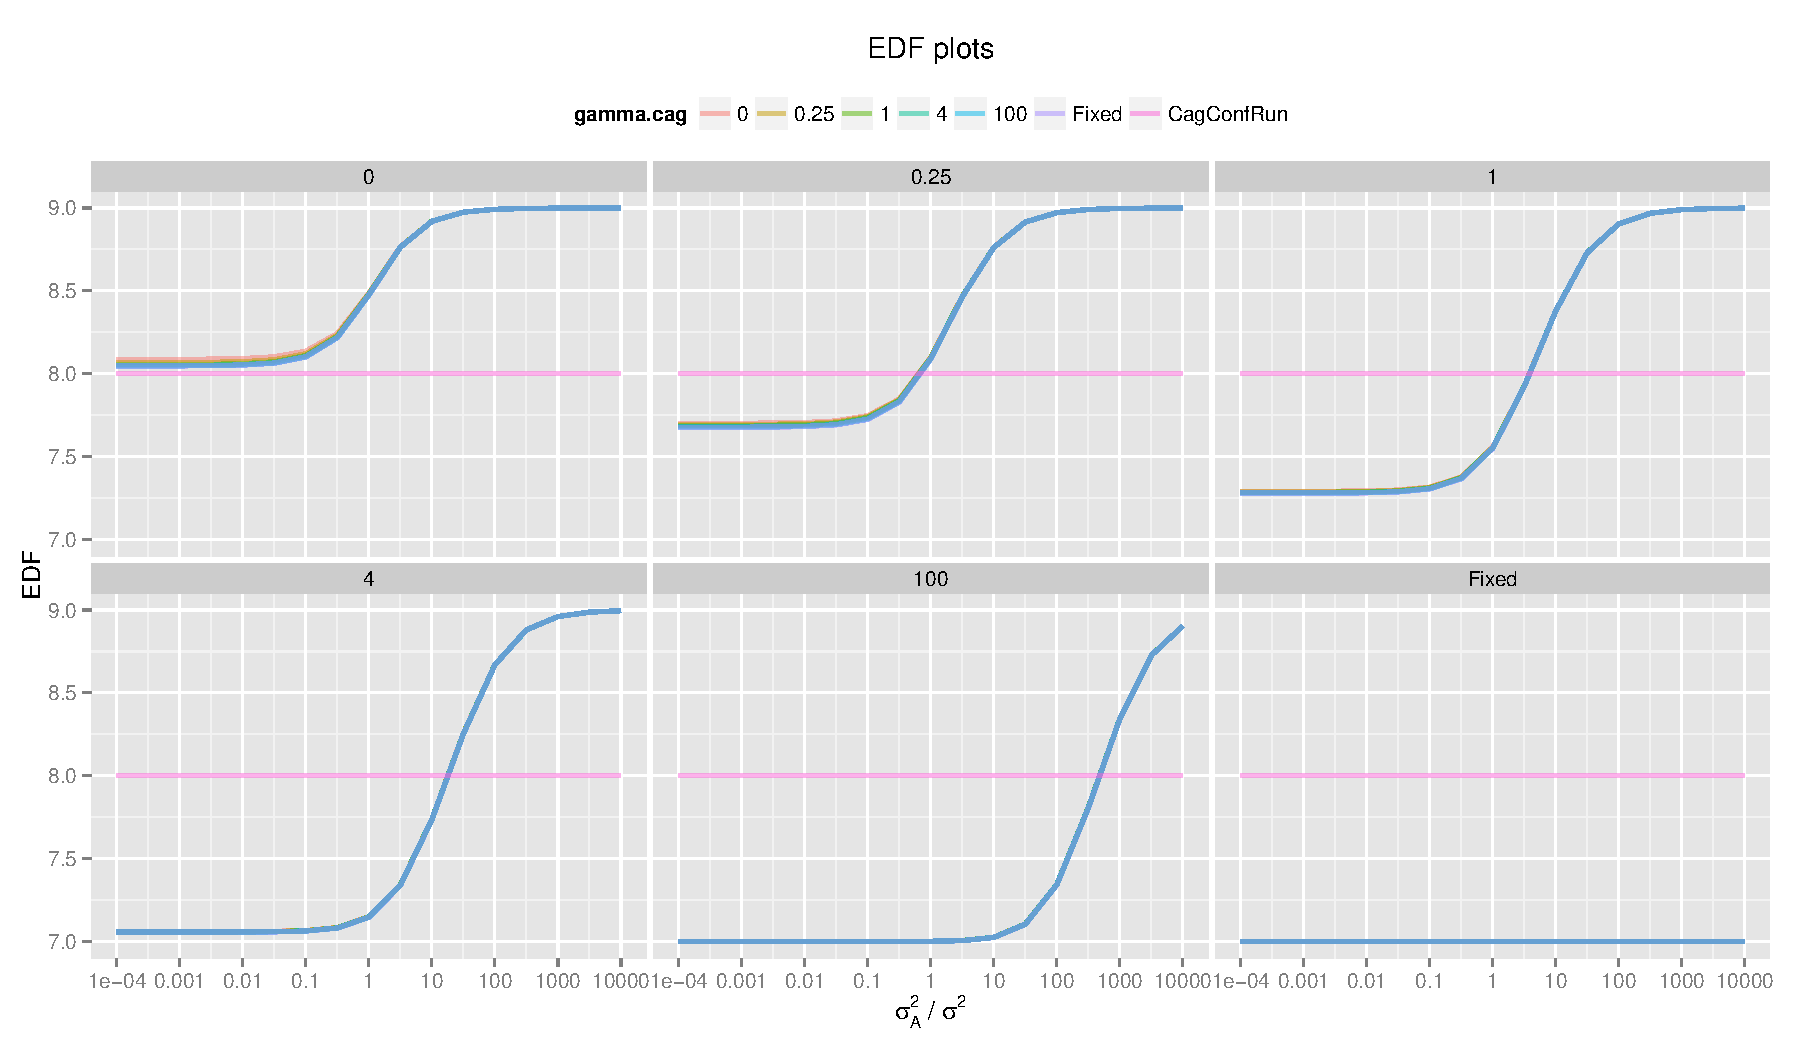
\includegraphics[width=1 \textwidth]{Graph/RBD442Tag4EDF.pdf}
\caption{Plots of EDF for the RCBD experiments with $v = 4, r_b = 4$ and $n_B = 4$, comparing different Between Cages VCs estimates as between an initial design where cages are confounded more with tags and one where cages are confounded more with runs, with Phase 2 experiment using 4 tags}
\label{fig:RCBD442Tag4EDF}
\end{figure}

Figure~\ref{fig:RCBD442Tag4EDFRun0} focuses on the situation where the Between Runs VCs are zero, as in Figure~\ref{fig:RCBD442Tag4EDF}. Notably, the EDF are highest when the Between Cages VCs are zero; however, the differences in EDF from different Between Cages VCs are too small to affect the power of the test.    

\begin{figure}[h!]
\centering
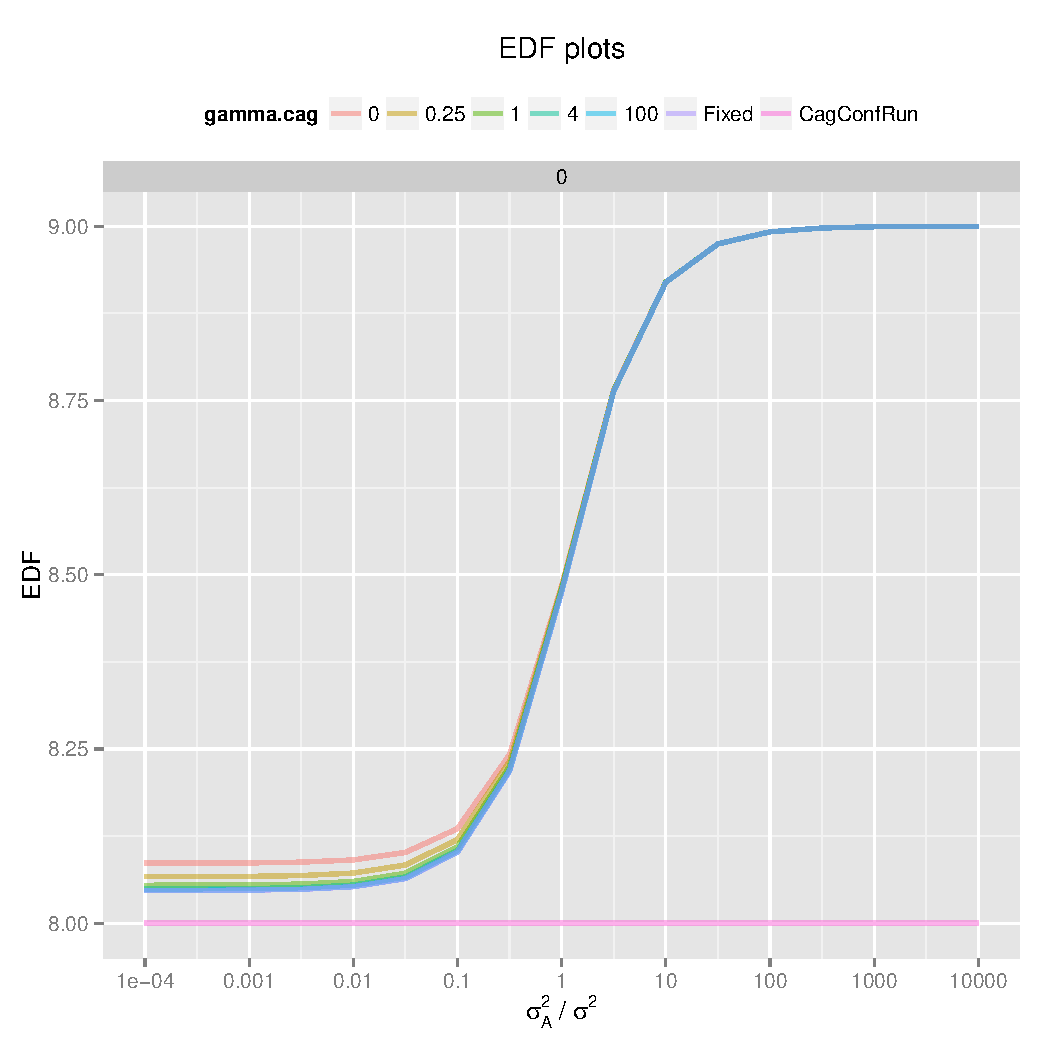
\includegraphics[width=.6 \textwidth]{Graph/RBD442Tag4EDFRun0.pdf}
\caption{Plots of EDF where the Between Runs VCs is zero for the RCBD experiments with $v = 4, r_b = 4$ and $n_B = 4$ comparing different Between Cages VCs estimates as between an initial design where cages are confounded more with tags, and one where cages are confounded more with runs}
\label{fig:RCBD442Tag4EDFRun0}
\end{figure}

Comparing the initial designs with the four-plex experiment, the design where cages are confounded more with runs has better EDF when Between Animals VCs are low and Between Runs VCs are high, because the EDF are always 8. If the VCs Between Animals are high and the Between Runs is low, the design where cages are confounded more with tags should be considered, as the EDF can be as high as 9.

Figure~\ref{fig:RCBD442Tag4vsTag8} includes the EDF from the eight-plex experiments and compares the EDF among the four designs. The two straight lines represent EDF fixed at $8$ and $7$ from the designs where cages are confounded more with runs in four-plex and eight-plex experiments, respectively. Hence, no animal information can be recovered from the Between Runs stratum. As for the designs where cage effects are confounded more with tag effects, the EDF can be as high as 9, because the animal information can be recovered from the Between Run stratum. Among these four designs, the one in which cage effects are confounded more with tags and using the eight-plex experiment is better, because the EDF are at least 8 under different VCs, and can reach up to 9 as the Between Animals VCs increase.    

\begin{figure}[h!]
\centering
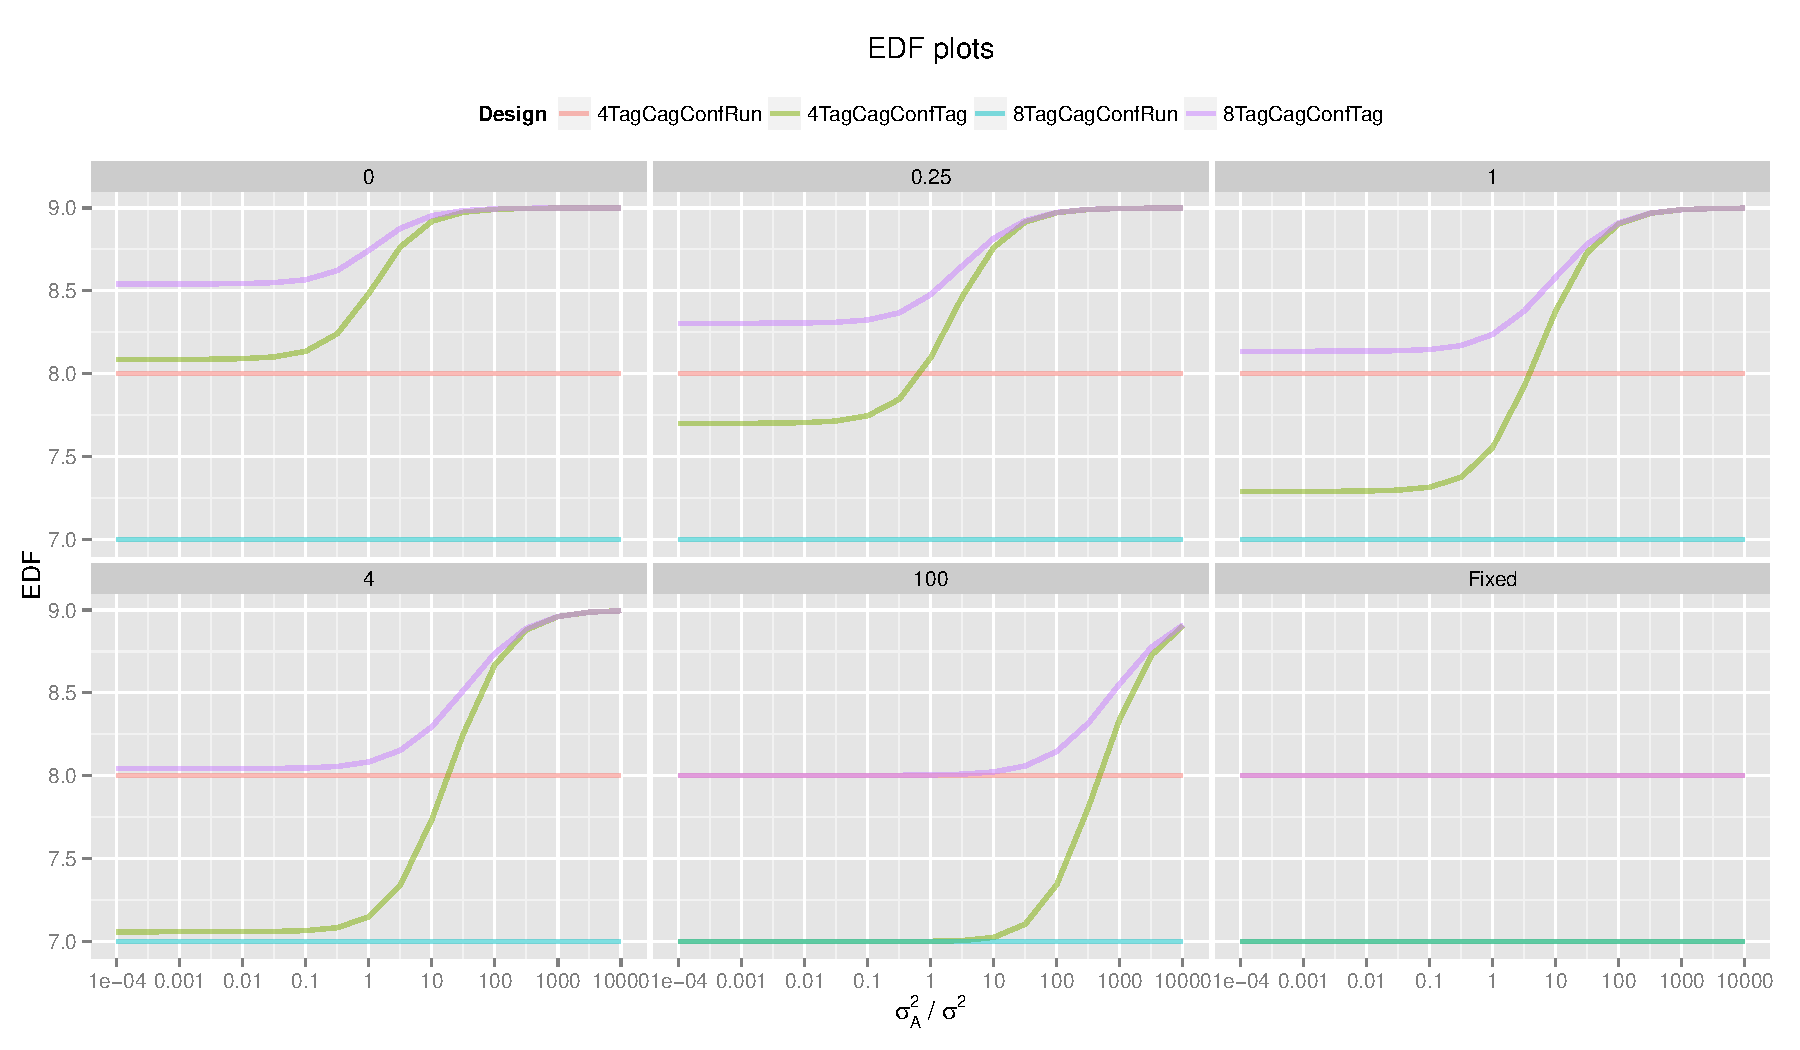
\includegraphics[width=1 \textwidth]{Graph/RBD442Tag4vsTag8.pdf}
\caption{Plots of EDF for RCBD experiments with $v = 4, r_b = 4$ and $n_B = 4$, comparing both the initial designs and the four-plex and eight-plex experiments}
\label{fig:RCBD442Tag4vsTag8}
\end{figure}

This section shows that cage allocation affects EDF. If the number of cages is even, using the design in which the cage effects are confounded more with tag effects is better, because it allows more DF to be associated with tag effects in the Between Cages stratum. Thus, it maximises the overall DF associated with the Between Animals Within Cages stratum in both the Between and Within Runs strata. However, if the cage number is odd, the guidelines followed in cases where the Phase 1 experiment is CRD can be used instead.  

The previous section showed that the experiments with the four-plex system generally have 1 DF associated with tag effects in the Between Animals Within Runs stratum, whereas those with the eight-plex system generally have 3 DF associated with tag effect in the Between Animals stratum. The eight-plex experiments can have higher EDF than the four-plex experiments only in situations involving 4 or 8 cages. This is because the cages can confound all 3 DF of the tag effects and maximise the overall DF associated in the Between Animals Within Cages stratum, as shown from the example given. As for experiments involving an even number of cages,  the four-plex system should be considered. 

%I found that the VCs Between Cages does not affect the EDF. This is because the animals are nested from cages, and thus when the EMS consists of VCs of Between Cages, it should also consist of between animal VCs.
%More specifically, when using experiments that involve even numbers of cages, but not those with 4 or 8 cages, the four-plex system is better than the eight-plex system. This is because only 1 DF associated with cages can be confounded with the tag effects. If the four-plex system is used, it is possible to confound the cages with the 1 DF associated with the tag effects, in which case the animals are then orthogonal to tags. If the eight-plex system is used, at least 2 DF are associated with the tag effects in the Between Animals Within Cages Within Runs stratum - e.g. $v = 2, r_b = 6, n_B  = 2, n_\gamma = 4$, where EDF is between 7 and 9. Moreover, $n_\gamma = 8$, where EDF is between 6 and 7. 

\section{Comparing the EDF when Phase 1 experiment is BIBD}
The case where the Phase 1 experiment is BIBD follows the same guidelines as in the previous sections. Despite the Between Cages stratum having some treatment information, the cages can still be allocated to confound more with either tags or runs. 

As for the experiments comparing 4 and 8 treatments, the eight-plex experiment is better than the four-plex experiment, because these two experiments use 4 and 8 cages, respectively.  

As for the experiments comparing 5 and 7 treatments, since they do not use an even number of cages, the guideline of CRD is used, which means the four-plex experiment genereates higher EDF than the eight-plex experiment. 

\section{Summary and Conclusion}
\label{sec:conclusion}
This chapter has presented the LC and REML methods for estimating the VCs. With the given VCs estimates, the method used to derive the EDF has then been shown. The EDF is important because it is associated with the residual MS in the stratum where the tests for treatment effects are conducted. 

The EDF are then compared between different optimal designs found where the Phase 1 experiment is arranged in CRD, RCBD and BIBD. When the Phase 1 experiment is arranged in CRD, the EDF are better when using the four-plex system than the eight-plex system, because the four-plex system contributes fewer DF associated with tag effects within the Between Animals Within Runs stratum. The eight-plex system is only better when comparing 8 tags because the treatment does not confound with animals in the Between Runs stratum. 

When the Phase 1 experiment uses RCBD or BIBD, the four-plex systems still tend to have higher EDF. Meanwhile, the eight-plex system is better when comparing eight treatments, for the reasons described in the example with CRD. The Phase 1 experiment also introduces an additional cage component. The RCBD example in Section~\ref{sec:expRCBD} shows that it is best to allocate the cages that are confounded more with tags, because this minimises the confounding of the animals with tags. Furthermore, when the Phase 1 experiment involves 4 or 8 cages, the eight-plex system is shown to be best, as in the example presented the cages completely confounded 3 DF associated with tag effects that were in the Between Animals stratum.   

This chapter only presented the recovery of random information from the Between Runs stratum, but it is also possible to recover treatment information. The optimal designs found for all cases have at least $80\%$ of the treatment average efficiency factor for estimating the treatment effects. Hence, recovery of treatment information from the Between Runs stratum is unnecessary.

%The R function getVcEDF() for estimating the VCs and the EDF has developed.

\bibliographystyle{plainnat}
\bibliography{ref}

\end{document}
